% Options for packages loaded elsewhere
\PassOptionsToPackage{unicode}{hyperref}
\PassOptionsToPackage{hyphens}{url}
\PassOptionsToPackage{dvipsnames,svgnames,x11names}{xcolor}
%
\documentclass[
  letterpaper,
  DIV=11,
  numbers=noendperiod]{scrreprt}

\usepackage{amsmath,amssymb}
\usepackage{lmodern}
\usepackage{iftex}
\ifPDFTeX
  \usepackage[T1]{fontenc}
  \usepackage[utf8]{inputenc}
  \usepackage{textcomp} % provide euro and other symbols
\else % if luatex or xetex
  \usepackage{unicode-math}
  \defaultfontfeatures{Scale=MatchLowercase}
  \defaultfontfeatures[\rmfamily]{Ligatures=TeX,Scale=1}
\fi
% Use upquote if available, for straight quotes in verbatim environments
\IfFileExists{upquote.sty}{\usepackage{upquote}}{}
\IfFileExists{microtype.sty}{% use microtype if available
  \usepackage[]{microtype}
  \UseMicrotypeSet[protrusion]{basicmath} % disable protrusion for tt fonts
}{}
\makeatletter
\@ifundefined{KOMAClassName}{% if non-KOMA class
  \IfFileExists{parskip.sty}{%
    \usepackage{parskip}
  }{% else
    \setlength{\parindent}{0pt}
    \setlength{\parskip}{6pt plus 2pt minus 1pt}}
}{% if KOMA class
  \KOMAoptions{parskip=half}}
\makeatother
\usepackage{xcolor}
\setlength{\emergencystretch}{3em} % prevent overfull lines
\setcounter{secnumdepth}{5}
% Make \paragraph and \subparagraph free-standing
\ifx\paragraph\undefined\else
  \let\oldparagraph\paragraph
  \renewcommand{\paragraph}[1]{\oldparagraph{#1}\mbox{}}
\fi
\ifx\subparagraph\undefined\else
  \let\oldsubparagraph\subparagraph
  \renewcommand{\subparagraph}[1]{\oldsubparagraph{#1}\mbox{}}
\fi


\providecommand{\tightlist}{%
  \setlength{\itemsep}{0pt}\setlength{\parskip}{0pt}}\usepackage{longtable,booktabs,array}
\usepackage{calc} % for calculating minipage widths
% Correct order of tables after \paragraph or \subparagraph
\usepackage{etoolbox}
\makeatletter
\patchcmd\longtable{\par}{\if@noskipsec\mbox{}\fi\par}{}{}
\makeatother
% Allow footnotes in longtable head/foot
\IfFileExists{footnotehyper.sty}{\usepackage{footnotehyper}}{\usepackage{footnote}}
\makesavenoteenv{longtable}
\usepackage{graphicx}
\makeatletter
\def\maxwidth{\ifdim\Gin@nat@width>\linewidth\linewidth\else\Gin@nat@width\fi}
\def\maxheight{\ifdim\Gin@nat@height>\textheight\textheight\else\Gin@nat@height\fi}
\makeatother
% Scale images if necessary, so that they will not overflow the page
% margins by default, and it is still possible to overwrite the defaults
% using explicit options in \includegraphics[width, height, ...]{}
\setkeys{Gin}{width=\maxwidth,height=\maxheight,keepaspectratio}
% Set default figure placement to htbp
\makeatletter
\def\fps@figure{htbp}
\makeatother

\usepackage{booktabs}
\usepackage{longtable}
\usepackage{array}
\usepackage{multirow}
\usepackage{wrapfig}
\usepackage{float}
\usepackage{colortbl}
\usepackage{pdflscape}
\usepackage{tabu}
\usepackage{threeparttable}
\usepackage{threeparttablex}
\usepackage[normalem]{ulem}
\usepackage{makecell}
\usepackage{xcolor}
\KOMAoption{captions}{tableheading}
\makeatletter
\@ifpackageloaded{tcolorbox}{}{\usepackage[many]{tcolorbox}}
\@ifpackageloaded{fontawesome5}{}{\usepackage{fontawesome5}}
\definecolor{quarto-callout-color}{HTML}{909090}
\definecolor{quarto-callout-note-color}{HTML}{0758E5}
\definecolor{quarto-callout-important-color}{HTML}{CC1914}
\definecolor{quarto-callout-warning-color}{HTML}{EB9113}
\definecolor{quarto-callout-tip-color}{HTML}{00A047}
\definecolor{quarto-callout-caution-color}{HTML}{FC5300}
\definecolor{quarto-callout-color-frame}{HTML}{acacac}
\definecolor{quarto-callout-note-color-frame}{HTML}{4582ec}
\definecolor{quarto-callout-important-color-frame}{HTML}{d9534f}
\definecolor{quarto-callout-warning-color-frame}{HTML}{f0ad4e}
\definecolor{quarto-callout-tip-color-frame}{HTML}{02b875}
\definecolor{quarto-callout-caution-color-frame}{HTML}{fd7e14}
\makeatother
\makeatletter
\makeatother
\makeatletter
\@ifpackageloaded{bookmark}{}{\usepackage{bookmark}}
\makeatother
\makeatletter
\@ifpackageloaded{caption}{}{\usepackage{caption}}
\AtBeginDocument{%
\ifdefined\contentsname
  \renewcommand*\contentsname{Table of contents}
\else
  \newcommand\contentsname{Table of contents}
\fi
\ifdefined\listfigurename
  \renewcommand*\listfigurename{List of Figures}
\else
  \newcommand\listfigurename{List of Figures}
\fi
\ifdefined\listtablename
  \renewcommand*\listtablename{List of Tables}
\else
  \newcommand\listtablename{List of Tables}
\fi
\ifdefined\figurename
  \renewcommand*\figurename{Figure}
\else
  \newcommand\figurename{Figure}
\fi
\ifdefined\tablename
  \renewcommand*\tablename{Table}
\else
  \newcommand\tablename{Table}
\fi
}
\@ifpackageloaded{float}{}{\usepackage{float}}
\floatstyle{ruled}
\@ifundefined{c@chapter}{\newfloat{codelisting}{h}{lop}}{\newfloat{codelisting}{h}{lop}[chapter]}
\floatname{codelisting}{Listing}
\newcommand*\listoflistings{\listof{codelisting}{List of Listings}}
\makeatother
\makeatletter
\@ifpackageloaded{caption}{}{\usepackage{caption}}
\@ifpackageloaded{subcaption}{}{\usepackage{subcaption}}
\makeatother
\makeatletter
\@ifpackageloaded{tcolorbox}{}{\usepackage[many]{tcolorbox}}
\makeatother
\makeatletter
\@ifundefined{shadecolor}{\definecolor{shadecolor}{rgb}{.97, .97, .97}}
\makeatother
\makeatletter
\makeatother
\ifLuaTeX
  \usepackage{selnolig}  % disable illegal ligatures
\fi
\IfFileExists{bookmark.sty}{\usepackage{bookmark}}{\usepackage{hyperref}}
\IfFileExists{xurl.sty}{\usepackage{xurl}}{} % add URL line breaks if available
\urlstyle{same} % disable monospaced font for URLs
\hypersetup{
  pdftitle={Richmond Regional Housing Framework Data Update},
  pdfauthor={HDAdvisors},
  colorlinks=true,
  linkcolor={blue},
  filecolor={Maroon},
  citecolor={Blue},
  urlcolor={Blue},
  pdfcreator={LaTeX via pandoc}}

\title{Richmond Regional Housing Framework Data Update}
\author{HDAdvisors}
\date{2022-09-09T00:00:00-04:00}

\begin{document}
\maketitle
\ifdefined\Shaded\renewenvironment{Shaded}{\begin{tcolorbox}[borderline west={3pt}{0pt}{shadecolor}, enhanced, interior hidden, breakable, frame hidden, sharp corners, boxrule=0pt]}{\end{tcolorbox}}\fi

\renewcommand*\contentsname{Table of contents}
{
\hypersetup{linkcolor=}
\setcounter{tocdepth}{2}
\tableofcontents
}
\bookmarksetup{startatroot}

\hypertarget{about}{%
\chapter*{About}\label{about}}
\addcontentsline{toc}{chapter}{About}

\begin{tcolorbox}[enhanced jigsaw, colback=white, colbacktitle=quarto-callout-note-color!10!white, bottomrule=.15mm, opacitybacktitle=0.6, colframe=quarto-callout-note-color-frame, breakable, opacityback=0, bottomtitle=1mm, titlerule=0mm, coltitle=black, leftrule=.75mm, left=2mm, title=\textcolor{quarto-callout-note-color}{\faInfo}\hspace{0.5em}{Note}, toptitle=1mm, arc=.35mm, rightrule=.15mm, toprule=.15mm]
This report is currently in development. It was last updated on
\textbf{2022-09-09}.
\end{tcolorbox}

This report is a data update for the Richmond Regional Housing
Framework, which was
\href{https://pharva.com/framework/about-the-framework/}{released} by
the Partnership for Housing Affordability (PHA) in January 2020. It will
support PHA's ongoing efforts to educate both decision-makers and the
public at large about the region's housing needs and opportunities. Data
in the report will also help PHA continue to monitor, change, and
implement the policy solutions outlined in the Framework.

There are four parts in this report:

\begin{enumerate}
\def\labelenumi{\arabic{enumi}.}
\tightlist
\item
  Demographic and socioeconomic changes
\item
  Housing supply and market changes
\item
  Gap analysis
\item
  Local summaries
\end{enumerate}

\hypertarget{how-to-read-this-report}{%
\section*{How to read this report}\label{how-to-read-this-report}}
\addcontentsline{toc}{section}{How to read this report}

This report is an interactive website with three main columns for
navigation:

\begin{enumerate}
\def\labelenumi{\arabic{enumi}.}
\tightlist
\item
  \textbf{Table of contents} (\emph{left}): Search bar and links to all
  chapters in the report.
\item
  \textbf{Current chapter} (\emph{center}): Main chapter content.
\item
  \textbf{On this page} (\emph{right}): Links to subsections within the
  currently-viewed chapter.
\end{enumerate}

Links to both the previous and next chapter are included at the bottom
of each chapter page.

\hypertarget{how-to-provide-feedback-on-this-draft}{%
\section*{How to provide feedback on this
draft}\label{how-to-provide-feedback-on-this-draft}}
\addcontentsline{toc}{section}{How to provide feedback on this draft}

All comments, questions, and suggestions should be emailed to
\href{mailto:jonathan@hdadvisors.net}{\nolinkurl{jonathan@hdadvisors.net}}
and \href{mailto:eric@hdadvisors.net}{\nolinkurl{eric@hdadvisors.net}}.

When applicable, please reference:

\begin{itemize}
\tightlist
\item
  The chapter number (``Chapter 3'')
\item
  The section/subsection (``3.2.1'')
\item
  The figure/title number (``Figure 3.3'')
\end{itemize}

\href{mailto:jonathan@hdadvisors.net,eric@hdadvisors.net}{Click here} to
generate an email in your inbox with the recipients auto-filled.

\hypertarget{changelog}{%
\section*{Changelog}\label{changelog}}
\addcontentsline{toc}{section}{Changelog}

\hypertarget{release-0.2}{%
\subsection*{Release 0.2}\label{release-0.2}}
\addcontentsline{toc}{subsection}{Release 0.2}

\emph{2022-09-06}

Second partial draft. Migrate from Bookdown project to Quarto project.

\hypertarget{release-0.1}{%
\subsection*{Release 0.1}\label{release-0.1}}
\addcontentsline{toc}{subsection}{Release 0.1}

\emph{2022-08-30}

First partial draft. Test site rendering and hosting. PART 1 chapters
fully drafted. Remaining chapters in final production.

Next release will include:

\begin{itemize}
\tightlist
\item
  PART 2 chapters:

  \begin{itemize}
  \tightlist
  \item
    Rental
  \item
    Housing Assistance
  \item
    Naturally-occurring affordable housing
  \end{itemize}
\item
  PART 3 chapters:

  \begin{itemize}
  \tightlist
  \item
    Affordability of current housing stock
  \end{itemize}
\item
  PART 4 chapters:

  \begin{itemize}
  \tightlist
  \item
    Remaining local summaries
  \end{itemize}
\end{itemize}

Still to come:

\begin{itemize}
\tightlist
\item
  Standardize colors across visualizations to match PHA brand palette
\item
  Make selection of plots interactive
\item
  Add in dynamic links for all footnotes and citations
\item
  Improve formatting for call-out boxes
\item
  PDF version of full report and locality summaries
\end{itemize}

\part{PART 1: Demographic and socioeconomic changes}

\hypertarget{part-1-1}{%
\chapter{Population changes}\label{part-1-1}}

\hypertarget{total-population-growth}{%
\section{Total population growth}\label{total-population-growth}}

The Richmond region has continued to grow between 2016 and 2020---adding
a net of 41,457 residents across the four major localities. The most
populous locality, Chesterfield County, experienced a near eight percent
increase in its population during this timeframe.

\begin{figure}

{\centering 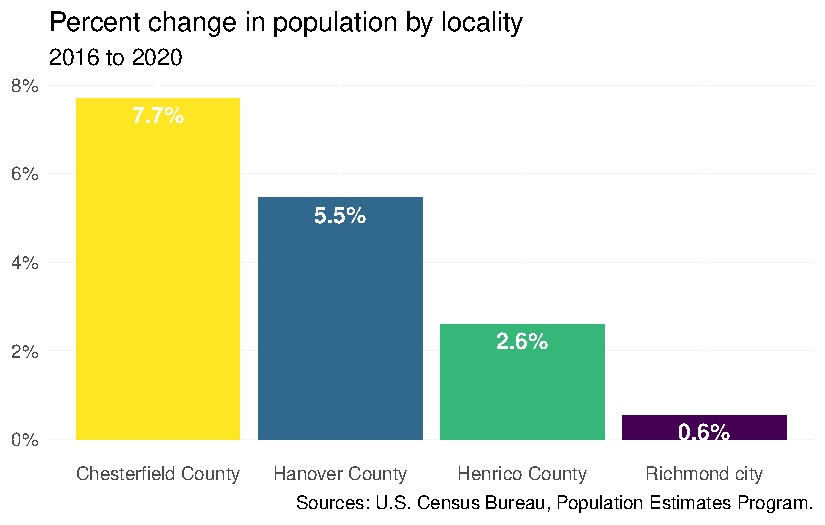
\includegraphics{./part-1-1_files/figure-pdf/fig-total-pop-plot-1.pdf}

}

\caption{\label{fig-total-pop-plot}Percent change in population by
locality}

\end{figure}

\hypertarget{components-of-population-change}{%
\section{Components of population
change}\label{components-of-population-change}}

In recent years, nearly two thirds of growth could be attributed to
either domestic or international migration into the region. But between
2020 and 2021, that share increased to over three quarters---reducing
the portion of the population growing due to natural increase to only 13
percent.

The region's growth continues to be driven primarily by new people
coming from other parts of the state and nation (64 percent of growth
between 2020 and 2021).

\begin{figure}

{\centering 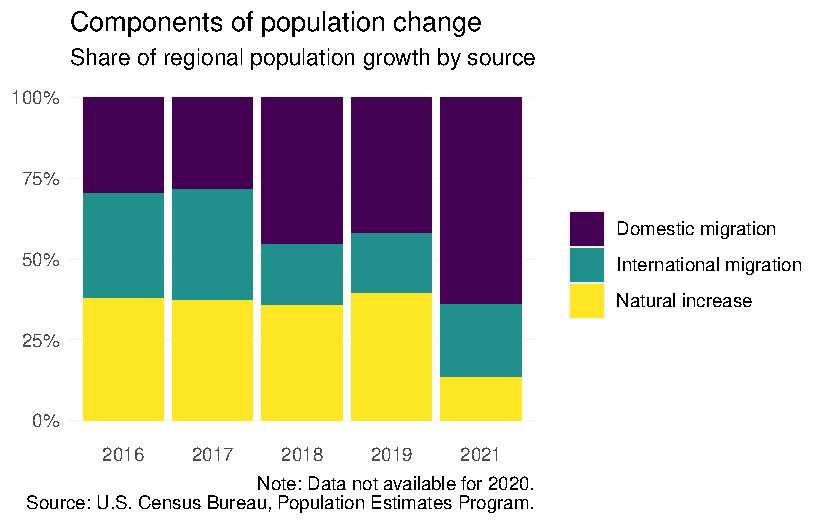
\includegraphics{./part-1-1_files/figure-pdf/fig-components-plot-1.pdf}

}

\caption{\label{fig-components-plot}Components of population change}

\end{figure}

\hypertarget{population-projections}{%
\section{Population projections}\label{population-projections}}

Between 2020 and 2050, the region is expected to grow by nearly a third
(29 percent)---reaching 1,338,306 residents.

\begin{figure}

{\centering 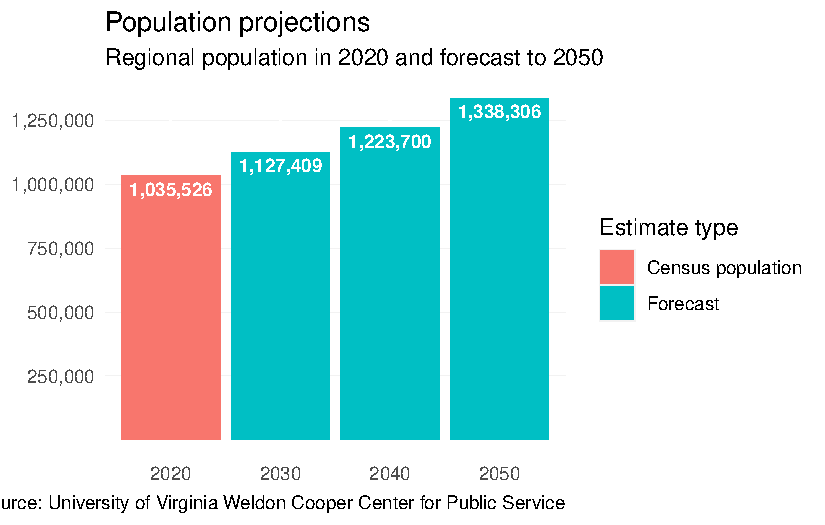
\includegraphics{./part-1-1_files/figure-pdf/fig-forecasts-region-plot-1.pdf}

}

\caption{\label{fig-forecasts-region-plot}Population projections}

\end{figure}

Over the next 30 years, Chesterfield County will continue to lead growth
across the region. By 2050, Chesterfield is expected to surpass half a
million residents, growing by 38 percent from the 2020 Census estimates.

Population growth trends will largely continue as they have with Hanover
County experiencing the second greatest growth from their 2020 estimates
(27 percent increase). Henrico County follows with a 26 percent increase
(+88,565), while the City of Richmond will only increase by about a
fifth (20 percent) over 30 years.

\begin{figure}

{\centering 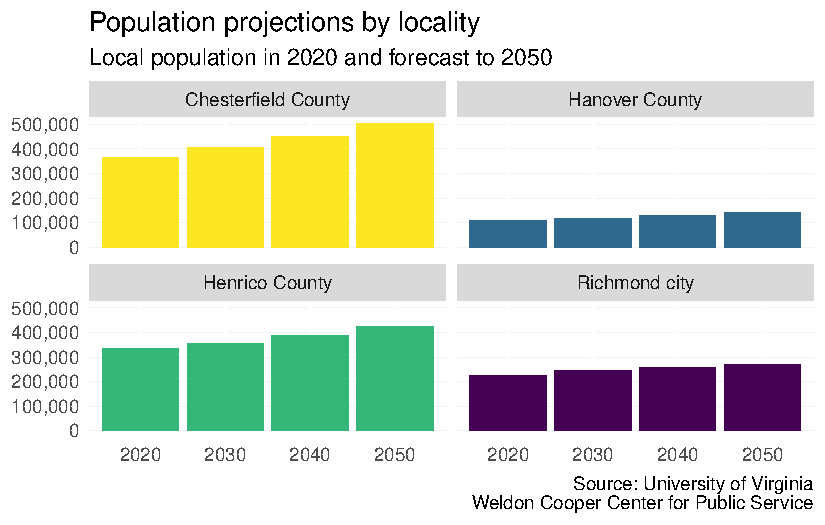
\includegraphics{./part-1-1_files/figure-pdf/fig-forecasts-locality-plot-1.pdf}

}

\caption{\label{fig-forecasts-locality-plot}Population projections by
locality}

\end{figure}

\hypertarget{part-1-2}{%
\chapter{Household characteristics}\label{part-1-2}}

\hypertarget{household-formation}{%
\section{Household formation}\label{household-formation}}

According to Census estimates, the region gained more than 15,000
households from 2016 to 2020. This growth was driven entirely by new
homeowners (17,436). Renter households, instead, saw much slower
increases from 2016 to 2019; from 2019 to 2020, the estimated number of
renters dropped more than 2,000 for a net loss of 609 over the full
period.

\begin{tcolorbox}[enhanced jigsaw, colback=white, colbacktitle=quarto-callout-warning-color!10!white, bottomrule=.15mm, opacitybacktitle=0.6, colframe=quarto-callout-warning-color-frame, breakable, opacityback=0, bottomtitle=1mm, titlerule=0mm, coltitle=black, leftrule=.75mm, left=2mm, title=\textcolor{quarto-callout-warning-color}{\faExclamationTriangle}\hspace{0.5em}{Warning}, toptitle=1mm, arc=.35mm, rightrule=.15mm, toprule=.15mm]
This anomalous data should be treated with caution. Lower American
Community Survey response rates during COVID-19 were most common among
lower-income and lower-educated households most likely to rent. Across
the Richmond region, overall ACS response rates
\href{https://www.prb.org/articles/capturing-covids-impact-on-the-american-community-survey-across-counties/}{declined
nearly 10 percent} from the 2015-2019 to 2016-2020 collection period.
\end{tcolorbox}

\begin{figure}

{\centering 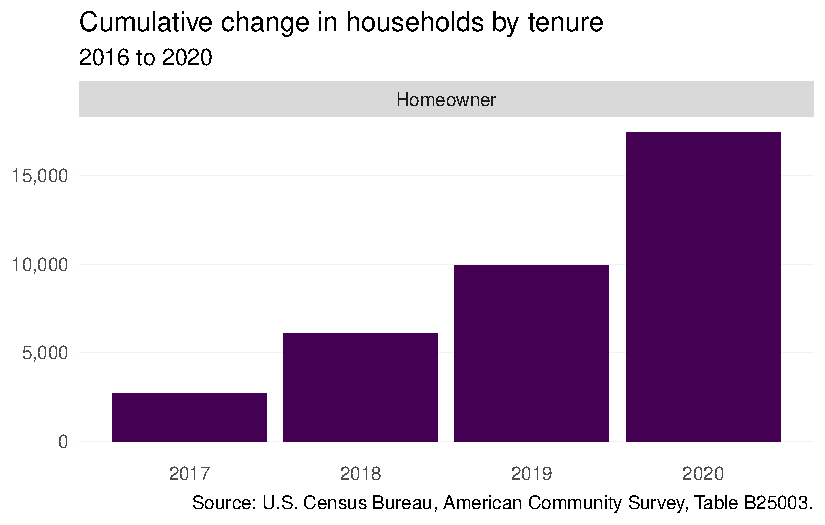
\includegraphics{./part-1-2_files/figure-pdf/fig-hh-form-plot-1.pdf}

}

\caption{\label{fig-hh-form-plot}Cumulative change in households by
tenure}

\end{figure}

\hypertarget{households-by-age}{%
\section{Households by age}\label{households-by-age}}

The single largest growing cohort of households across the region are
homeowners 65 years and over. Thanks in large part to youngest baby
boomers aging into retirement, this group increased by more than 13,000.
Younger homeowners saw much smaller gains.

Among renters, most growth occurred in senior householders. The
significant decrease of renter households under 25 (more than 3,200)
should be treated with caution, as this population likely had much lower
ACS response rates during COVID-19.

\begin{figure}

{\centering 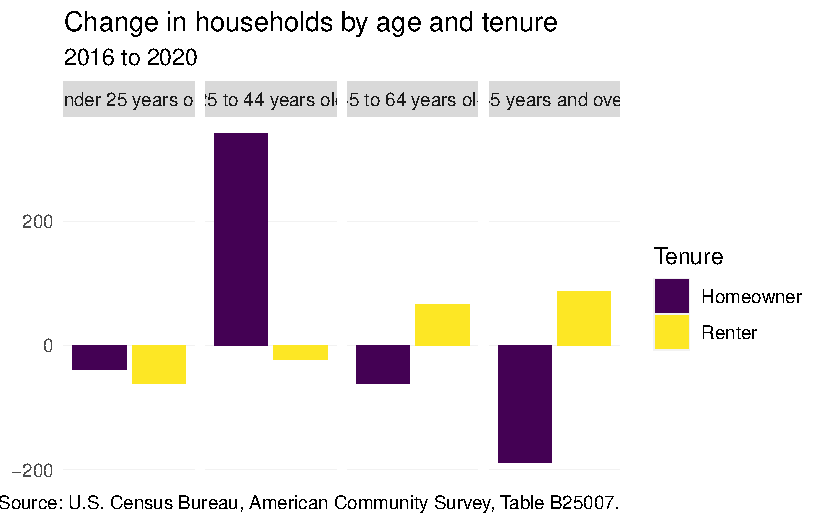
\includegraphics{./part-1-2_files/figure-pdf/fig-hh-age-plot-1.pdf}

}

\caption{\label{fig-hh-age-plot}Change in households by age and tenure}

\end{figure}

\hypertarget{households-by-type}{%
\section{Households by type}\label{households-by-type}}

Married-couple families continued to be the dominant household type in
the region, growing by 9,625 from 2016 to 2020. Living alone also become
more common, likely the result of seniors increasingly living on their
own. Households headed by single females were the only type to decline;
however, this could potentially be attributed to lower ACS response
rates among those households during COVID-19.

\begin{figure}

{\centering 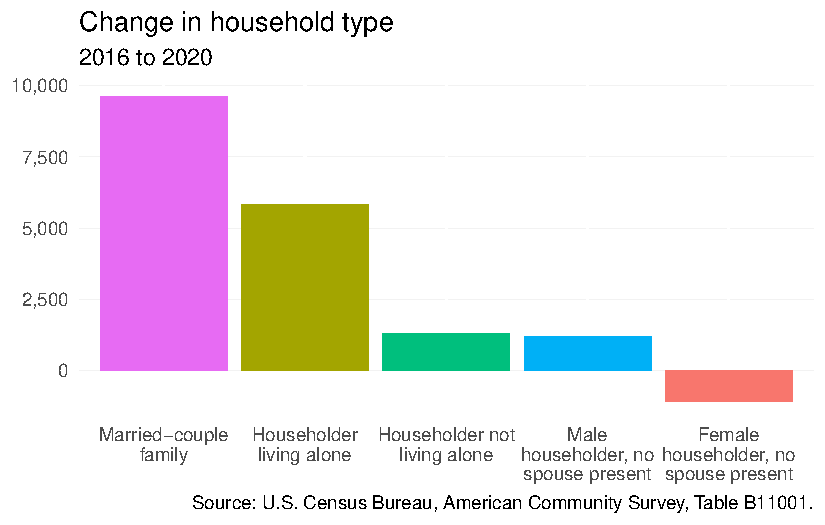
\includegraphics{./part-1-2_files/figure-pdf/fig-hh-type-plot-1.pdf}

}

\caption{\label{fig-hh-type-plot}Change in household type}

\end{figure}

\hypertarget{households-by-size}{%
\section{Households by size}\label{households-by-size}}

Two-person homeowning households were by and large the fastest-growing
cohort among different size households from 2016 to 2020. There was also
a significant increase in the number of homeowners living alone, as well
as homeowners with four-person households.

Persons living alone were the only size of renter households that grew
with any significance over this period. One potential explanation for
the notable decreases in the number of three- and four-person renter
households is lower ACS response rates among younger adults living with
roommates during COVID-19. This population, which does not include
college students living in dorms (``group quarters'' are not households
in Census methodology), was likely to move back home with parents during
the initial phases of the pandemic.

\begin{figure}

{\centering 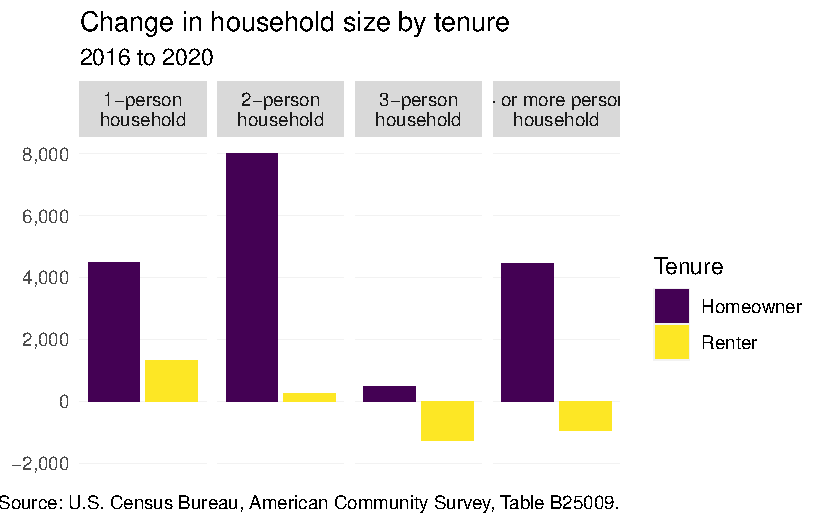
\includegraphics{./part-1-2_files/figure-pdf/fig-hh-size-plot-1.pdf}

}

\caption{\label{fig-hh-size-plot}Change in household size by tenure}

\end{figure}

\hypertarget{households-with-children}{%
\section{Households with children}\label{households-with-children}}

The number of homeowners without children in the region grew
significantly (by almost 9,000) from 2016 to 2020. This is likely due in
large part to baby boomer parents now living without their children. The
number of homeowners in nonfamily households also increased---driven
primarily by those now living alone. Families with children were the
least common group of homeowners that grew.

The only group of renters that saw significant growth was nonfamily
households. This includes both renters that live alone and those that
live with non-related roommates. The estimated number of renters with
children declined sharply; this may also be a symptom of lower pandemic
ACS responses among lower-income working families.

\begin{figure}

{\centering 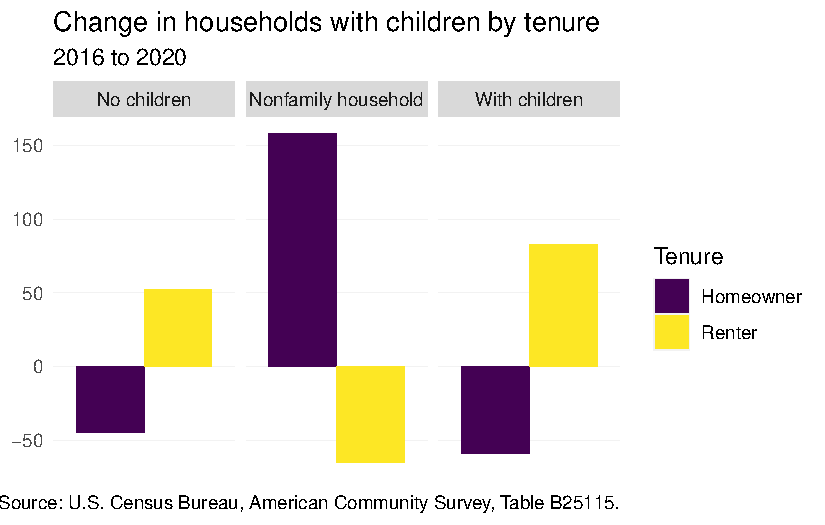
\includegraphics{./part-1-2_files/figure-pdf/fig-hh-child-plot-1.pdf}

}

\caption{\label{fig-hh-child-plot}Change in households with children by
tenure}

\end{figure}

\hypertarget{senior-living-arrangements}{%
\section{Senior living arrangements}\label{senior-living-arrangements}}

Since 2016, the region's senior population increased almost exclusively
among three types:

\begin{itemize}
\tightlist
\item
  Seniors who are the head of the household,
\item
  Seniors who are the spouse of the head of the households, and
\item
  Seniors who live alone.
\end{itemize}

The estimated number of seniors within group quarters (e.g.~nursing
homes, assisted living facilities) increased by less than 200. This
figure should be assessed in context of ACS collection
\href{https://www.census.gov/newsroom/blogs/random-samplings/2021/09/collecting-acs-data-from-group-quarters-amid-the-pandemic.html}{challenges}
in group quarters settings throughout the COVID-19 pandemic.

\begin{figure}

{\centering 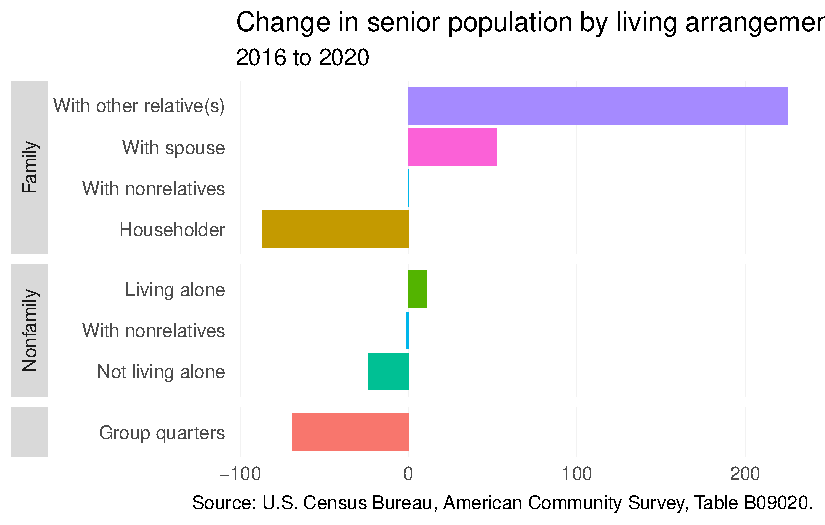
\includegraphics{./part-1-2_files/figure-pdf/fig-hh-seniors-plot-1.pdf}

}

\caption{\label{fig-hh-seniors-plot}Change in senior population by
living arrangement}

\end{figure}

\hypertarget{subfamilies}{%
\section{Subfamilies}\label{subfamilies}}

The Census Bureau defines a \emph{subfamily} as a group of related
individuals who live in the household of someone else. As of 2020, there
were approximately 9,850 subfamilies across the region. Two-thirds of
those are single mothers living with at least one child of their own.
These estimates have remained stable since 2016.

\begin{figure}

{\centering 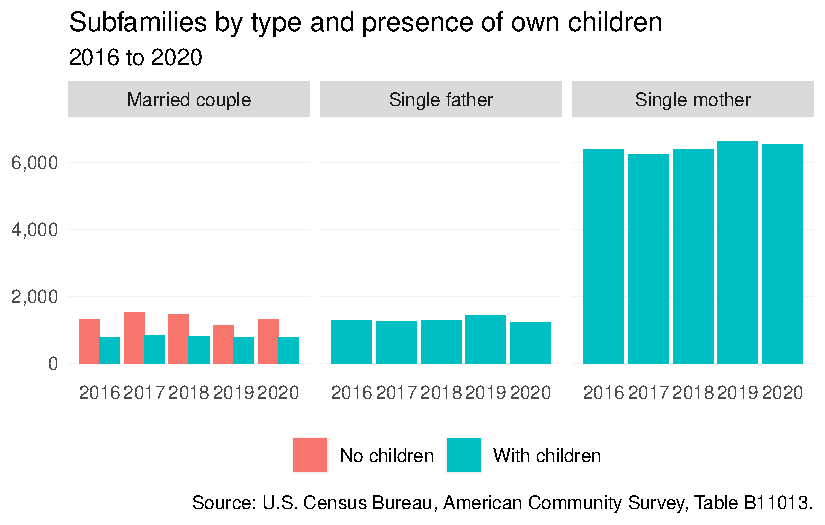
\includegraphics{./part-1-2_files/figure-pdf/fig-hh-subfam-plot-1.pdf}

}

\caption{\label{fig-hh-subfam-plot}Subfamilies by type and presence of
own children}

\end{figure}

\hypertarget{multigenerational-households}{%
\section{Multigenerational
households}\label{multigenerational-households}}

The Census Bureau defines \emph{multigenerational} households as those
with three or more generations. According to the Pew Research Center,
the share of the American population in multigenerational households
\href{https://www.pewresearch.org/social-trends/2022/03/24/the-demographics-of-multigenerational-households/}{increased}
from just 7 percent in 1971 to 18 percent in 2021.

However, multigenerational households in the Richmond region are less
common than the national average. As of 2020, the share of persons in
multiple generation households across the region has stayed between 7
and 8 percent from 2016 to 2020.

\begin{tcolorbox}[enhanced jigsaw, colback=white, colbacktitle=quarto-callout-note-color!10!white, bottomrule=.15mm, opacitybacktitle=0.6, colframe=quarto-callout-note-color-frame, breakable, opacityback=0, bottomtitle=1mm, titlerule=0mm, coltitle=black, leftrule=.75mm, left=2mm, title=\textcolor{quarto-callout-note-color}{\faInfo}\hspace{0.5em}{Note}, toptitle=1mm, arc=.35mm, rightrule=.15mm, toprule=.15mm]
Multigenerational households estimates are not available from the
standard ACS tables published by the Census Bureau. The data in this
section comes from the Public Use Microdata Sample (PUMS), which are
available only by special Public Use Microdata Areas (PUMAs) which
contain at least 100,000 people.

While PUMA boundaries align with Chesterfield County, Henrico County,
and Richmond city, the PUMA containing Hanover County also includes
Powhatan, Goochland, New Kent, King William, Charles City counties.
\end{tcolorbox}

Multigenerational households are slightly more common in the core metro
area (Chesterfield, Henrico, and Richmond) than the outlying suburbs.
The share of multigenerational households in Chesterfield and Richmond
appears to be decreasing slightly, while increasing slightly in the
outer counties. The share of Henrico's population in multigenerational
households continues to sit around 8 percent.

\begin{figure}

{\centering 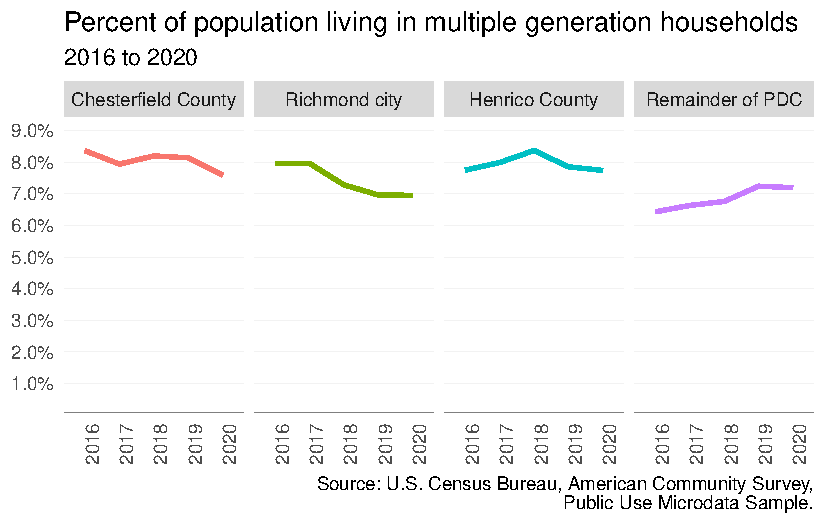
\includegraphics{./part-1-2_files/figure-pdf/fig-hh-multigen-plot-1.pdf}

}

\caption{\label{fig-hh-multigen-plot}Percent of population living in
multiple generation households}

\end{figure}

\hypertarget{adult-children-with-parents}{%
\section{Adult children with
parents}\label{adult-children-with-parents}}

Over the past decade, a common stereotype has been the adult millennial
child continuing to live with their parents. While this trope is based
in real economic challenges faced by young adults, such as increasing
housing costs and student debt, its magnitude can often be overstated.

Today, more than 75,800 adults 18 to 34 years old in the region---about
one-in-three---live with their parents. This is more than any other
arrangement. However, since 2016, the fastest growing living arrangement
for young adults has been with an unmarried partner, followed by other
nonrelatives (roommates). In fact, the share of young adults now living
with a married spouse increased slightly more than the share still
living with parents.

\begin{figure}

{\centering 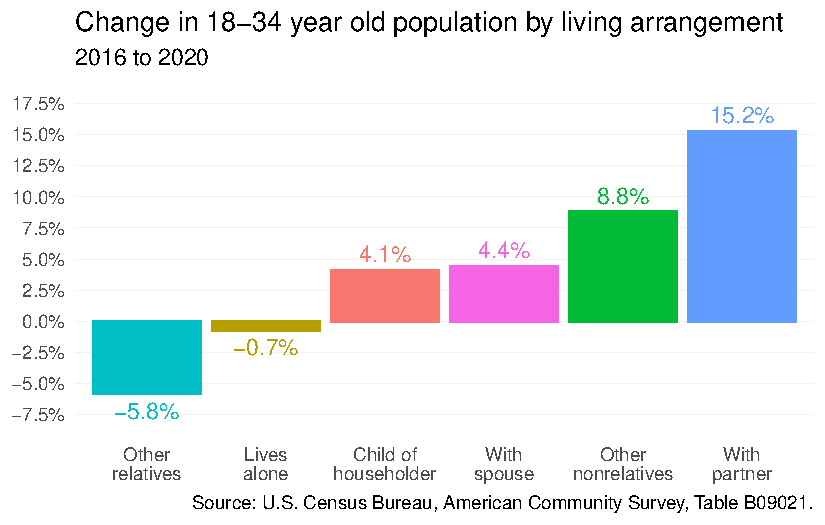
\includegraphics{./part-1-2_files/figure-pdf/fig-hh-adultchild-plot-1.pdf}

}

\caption{\label{fig-hh-adultchild-plot}Change in 18-34 year old
population by living arrangement}

\end{figure}

\hypertarget{part-1-3}{%
\chapter{Incomes and wages}\label{part-1-3}}

\hypertarget{household-incomes}{%
\section{Household incomes}\label{household-incomes}}

\hypertarget{incomes-by-tenure}{%
\subsection{Incomes by tenure}\label{incomes-by-tenure}}

From 2016 to 2020, the region saw large increases in the number of
six-figure income households, particularly among homeowners (well over
25,000), but also renters (almost 6,500). This growth can likely be
attributed to both new high-income residents from outside the region, as
well as income growth among households already in the region.

There was also a minor increase in the number of middle-income renters
earning between \$50,000 and \$100,000, reflecting continued demand for
new market-rate apartments---along with affordable starter homes.

\begin{figure}

{\centering 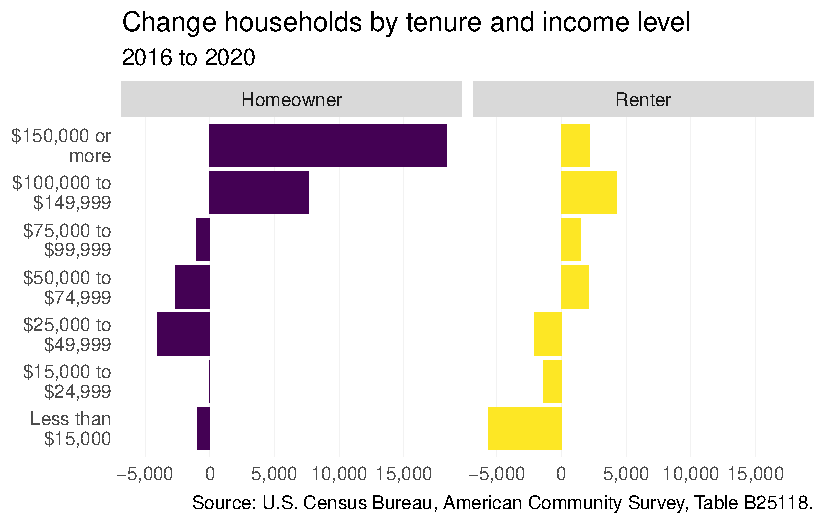
\includegraphics{./part-1-3_files/figure-pdf/fig-hh-inc-plot-1.pdf}

}

\caption{\label{fig-hh-inc-plot}Change households by tenure and income
level}

\end{figure}

Average homeowner incomes continue to be well above average renter
incomes across the region. When adjusted for inflation, incomes across
tenures for each locality show very minor to modest growth. Incomes in
the city---for both homeowners and renters---remain significantly below
those in the surrounding counties. The average household income for
homeowners in the counties is around three times that of renters in
Richmond.

\begin{figure}

{\centering 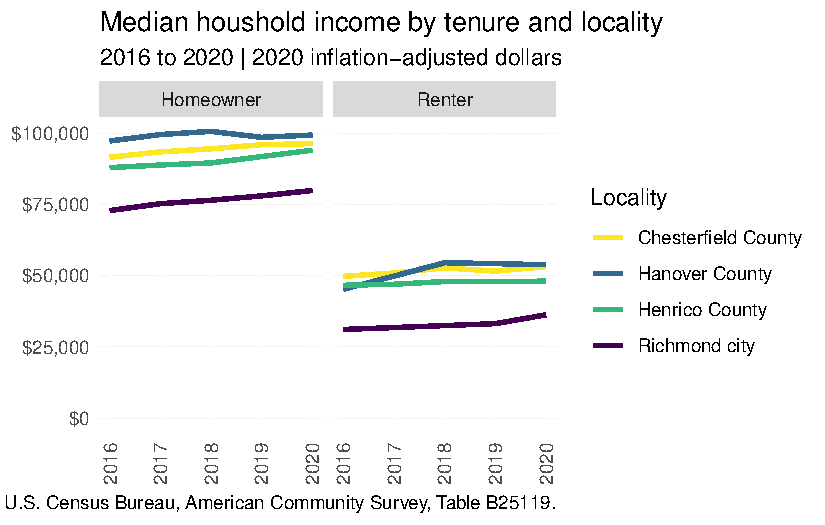
\includegraphics{./part-1-3_files/figure-pdf/fig-med-income-plot-1.pdf}

}

\caption{\label{fig-med-income-plot}Median houshold income by tenure and
locality}

\end{figure}

\hypertarget{incomes-by-race-and-ethnicity}{%
\subsection{Incomes by race and
ethnicity}\label{incomes-by-race-and-ethnicity}}

Average incomes in the region remain unequal by race and ethnicity.
Households with the highest incomes include Asian and white,
non-Hispanic residents in the counties---earning well above \$75,000.
Black and Hispanic households consistently have the lowest average
incomes, along with multiracial households in Henrico and Richmond.

\begin{figure}

{\centering 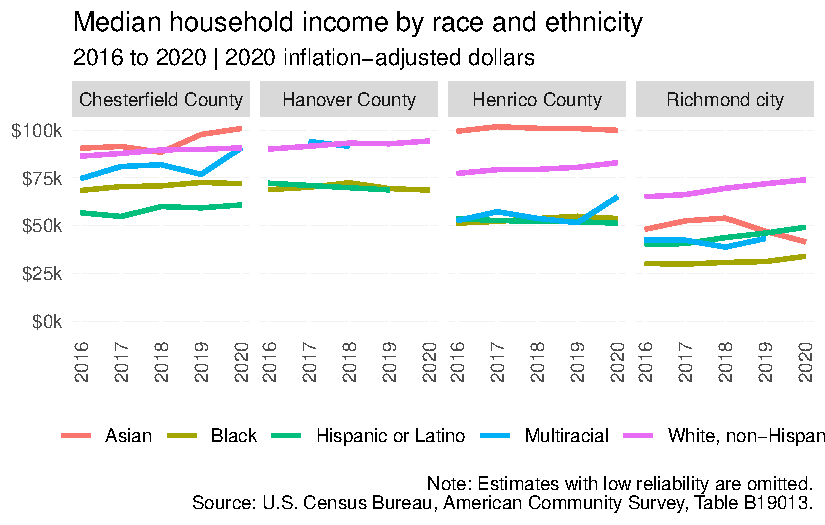
\includegraphics{./part-1-3_files/figure-pdf/fig-inc-race-plot-1.pdf}

}

\caption{\label{fig-inc-race-plot}Median household income by race and
ethnicity}

\end{figure}

\hypertarget{incomes-by-family-type}{%
\subsection{Incomes by family type}\label{incomes-by-family-type}}

Household incomes also vary by the presence of children or other related
individuals. Throughout the region, non-family households (i.e., persons
living alone or with unrelated persons) consistently have average
incomes below \$50,000. In Henrico and Chesterfield counties, families
living with and without children under 18 have very similar income
levels. This trend is different in Hanover, where families with children
have much higher incomes, as well as Richmond, where they have much
lower incomes.

\begin{figure}

{\centering 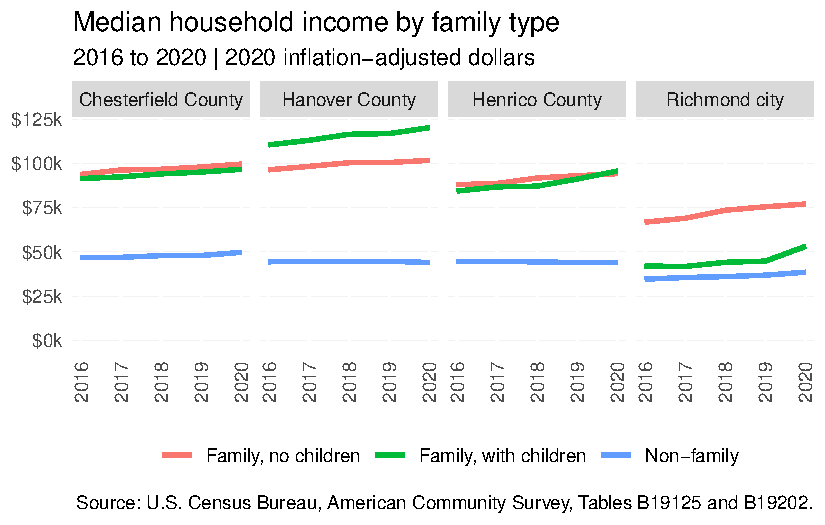
\includegraphics{./part-1-3_files/figure-pdf/fig-inc-child-plot-1.pdf}

}

\caption{\label{fig-inc-child-plot}Median household income by family
type}

\end{figure}

\hypertarget{wages}{%
\section{Wages}\label{wages}}

\begin{tcolorbox}[enhanced jigsaw, colback=white, colbacktitle=quarto-callout-note-color!10!white, bottomrule=.15mm, opacitybacktitle=0.6, colframe=quarto-callout-note-color-frame, breakable, opacityback=0, bottomtitle=1mm, titlerule=0mm, coltitle=black, leftrule=.75mm, left=2mm, title=\textcolor{quarto-callout-note-color}{\faInfo}\hspace{0.5em}{Note}, toptitle=1mm, arc=.35mm, rightrule=.15mm, toprule=.15mm]
Wage data in this section is sourced from the Occupational Employment
and Wage Statistics (OEWS) program of the Bureau of Labor Statistics.
OEWS is updated annually, most recently for 2021 data. This dataset
provides a rich look into wage distribution by industry and occupation.

However, OEWS is only available at the national, state, and metro
levels. Therefore, the data below covers the full Richmond, Virginia
Metropolitan Statistical Area (MSA) rather than the (smaller) PHA
region.
\end{tcolorbox}

\hypertarget{wage-change-by-percentile}{%
\subsection{Wage change by percentile}\label{wage-change-by-percentile}}

While regional wages increased across the board from May 2019 to May
2021, the largest percent increases in average wages were among jobs
that paid at and below the median wage. In fact, the largest growth
occurred in the lowest 10th percentile of wages, due in large part to
state lawmakers adopting incremental increases to Virginia's minimum
wage in 2020. The first increase from \$7.25 to \$9.50 per hour took
effect in 2021.

\begin{tcolorbox}[enhanced jigsaw, colback=white, colbacktitle=quarto-callout-note-color!10!white, bottomrule=.15mm, opacitybacktitle=0.6, colframe=quarto-callout-note-color-frame, breakable, opacityback=0, bottomtitle=1mm, titlerule=0mm, coltitle=black, leftrule=.75mm, left=2mm, title=\textcolor{quarto-callout-note-color}{\faInfo}\hspace{0.5em}{Note}, toptitle=1mm, arc=.35mm, rightrule=.15mm, toprule=.15mm]
Today, state minimum wage is \$11.00 per hour. Under
\href{https://lis.virginia.gov/cgi-bin/legp604.exe?201+sum+SB7}{current
law}, it will increase again to \$12.00 in 2023. Lawmakers must reenact
the measure by July 2024 to initiative further increases to \$15.00 per
hour by 2026.
\end{tcolorbox}

Another factor in this low-end wage growth is likely the
\href{https://www.bls.gov/opub/ted/2022/24-percent-of-establishments-increased-pay-or-paid-bonuses-because-of-covid-19-pandemic.htm}{increased
pay} offered by many businesses, especially in the food, retail, and
accommodation sectors, to encourage workers to return during the
COVID-19 recovery.

\begin{figure}

{\centering 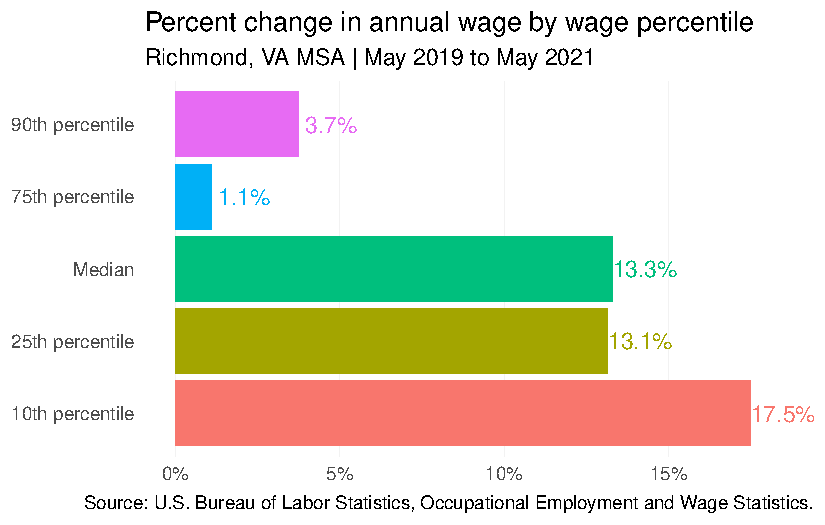
\includegraphics{./part-1-3_files/figure-pdf/fig-wage-pct-plot-1.pdf}

}

\caption{\label{fig-wage-pct-plot}Percent change in annual wage in
Richmond, VA MSA}

\end{figure}

\hypertarget{wage-change-by-occupation}{%
\subsection{Wage change by occupation}\label{wage-change-by-occupation}}

Over this same period, wages in the region grew for four of the five
most common occupation categories by total employment numbers. Workers
in the Transportation and Material Moving sector saw the largest
increases---from an average annual salary of \$30,250 to \$36,370 (over
20 percent).

Jobs in Food Preparation and Serving, Sales, and Business and Financial
Operations sectors---totaling more than 162,000 workers in the region as
of May 2021---also saw wage growth, but less than the 13.3 percent
average increase. Meanwhile, wages among Office and Administrative
Support positions remained nearly the same (-0.2 percent) from 2019 to
2021.

\begin{figure}

{\centering 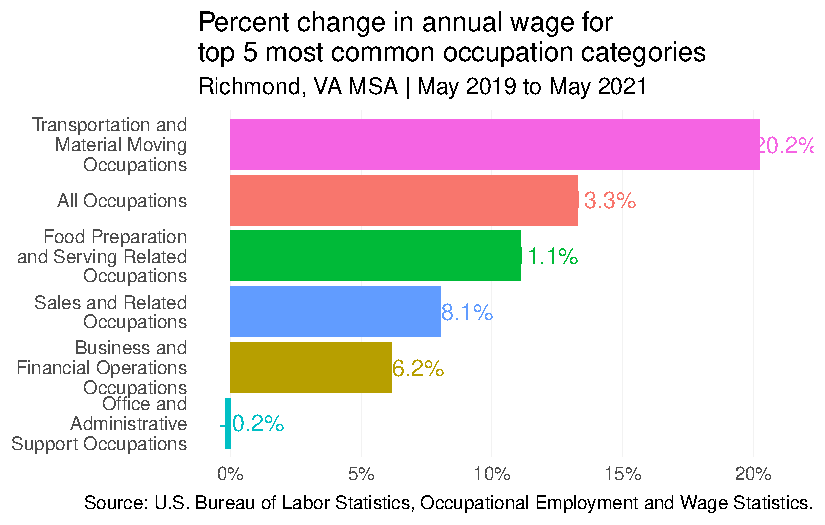
\includegraphics{./part-1-3_files/figure-pdf/fig-wage-occ-plot-1.pdf}

}

\caption{\label{fig-wage-occ-plot}Percent change in annual wage for top
5 most common occupation categories}

\end{figure}

\hypertarget{part-1-4}{%
\chapter{Special populations}\label{part-1-4}}

\hypertarget{independent-living-difficulty}{%
\section{Independent living
difficulty}\label{independent-living-difficulty}}

In the American Community Survey (ACS), the Census Bureau collects a
range of characteristics to capture the range of different disability
types found in the population. One important disability type available
in ACS data is \emph{independent living difficulty}, which includes
persons who:

\begin{quote}
\emph{Because of a physical, mental, or emotional problem, {[}have{]}
difficulty doing errands alone such as visiting a doctor's office or
shopping.}
\end{quote}

As a result, persons with these difficulties often face significant
housing challenges as well.

\hypertarget{by-age}{%
\subsection{By age}\label{by-age}}

From 2016 to 2020, the region added almost 2,600 more persons with
independent living difficulties. The largest increases occurred among
young adults under 35, as well as ``young'' seniors between 65 and 74.
The latter group will see their needs increase acutely in the next
decade as they continue to age and potentially become more dependent on
others.

\begin{figure}

{\centering 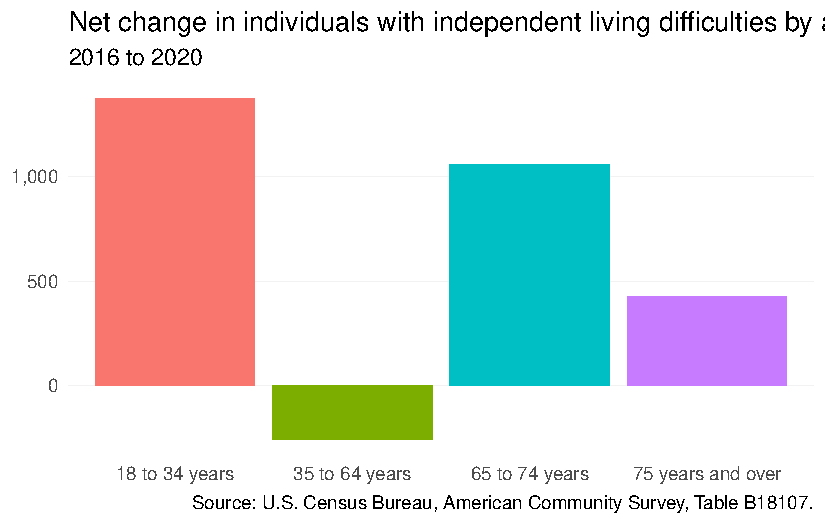
\includegraphics{./part-1-4_files/figure-pdf/fig-ind-liv-age-plot-1.pdf}

}

\caption{\label{fig-ind-liv-age-plot}Net change in individuals with
independent living difficulties by age}

\end{figure}

\hypertarget{by-tenure}{%
\subsection{By tenure}\label{by-tenure}}

\begin{tcolorbox}[enhanced jigsaw, colback=white, colbacktitle=quarto-callout-note-color!10!white, bottomrule=.15mm, opacitybacktitle=0.6, colframe=quarto-callout-note-color-frame, breakable, opacityback=0, bottomtitle=1mm, titlerule=0mm, coltitle=black, leftrule=.75mm, left=2mm, title=\textcolor{quarto-callout-note-color}{\faInfo}\hspace{0.5em}{Note}, toptitle=1mm, arc=.35mm, rightrule=.15mm, toprule=.15mm]
The detailed estimates for persons with independent living difficulties
in this and the next section are not available from the standard ACS
tables published by the Census Bureau. The data in these sections come
from the Public Use Microdata Sample (PUMS), which are available only by
special Public Use Microdata Areas (PUMAs) which contain at least
100,000 people.

While PUMA boundaries align with Chesterfield County, Henrico County,
and Richmond city, the PUMA containing Hanover County also includes
Powhatan, Goochland, New Kent, King William, Charles City counties.
\end{tcolorbox}

Nearly all persons with independent living difficulties throughout the
region live in regular homes, and not assisted living facilities or
other group quarters. Most are in homes that they own, or in homes owned
by another occupant, such as a spouse. This is not the case in Richmond,
however, where about half live in rented homes.

\begin{figure}

{\centering 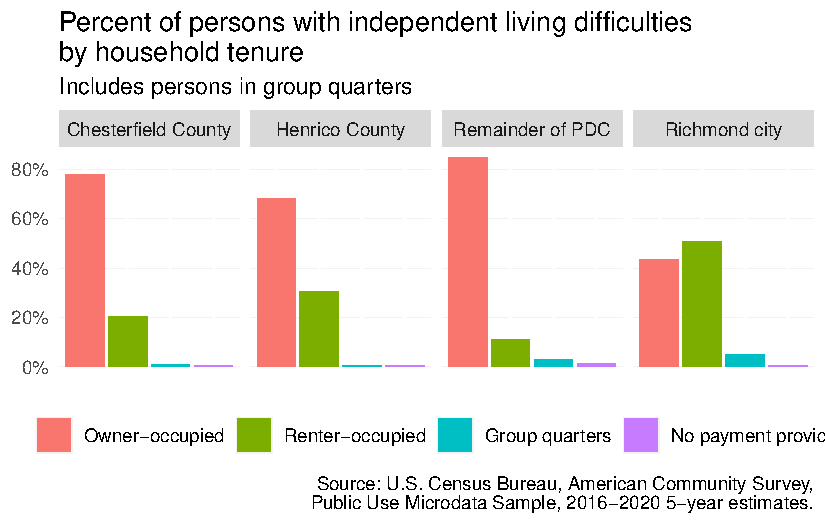
\includegraphics{./part-1-4_files/figure-pdf/fig-ind-liv-tenure-plot-1.pdf}

}

\caption{\label{fig-ind-liv-tenure-plot}Percent of persons with
independent living difficulties by household tenure}

\end{figure}

\hypertarget{by-household-size}{%
\subsection{By household size}\label{by-household-size}}

Persons with independent living difficulties are most likely to live
with one other person in their home. Slightly larger households (3 to 4
persons total) are also common. Still, more than 15 percent live
alone---including nearly one-in-four in Richmond. However, based on ACS
data collection methods, ``living alone'' also includes persons residing
in group quarters.

\begin{figure}

{\centering 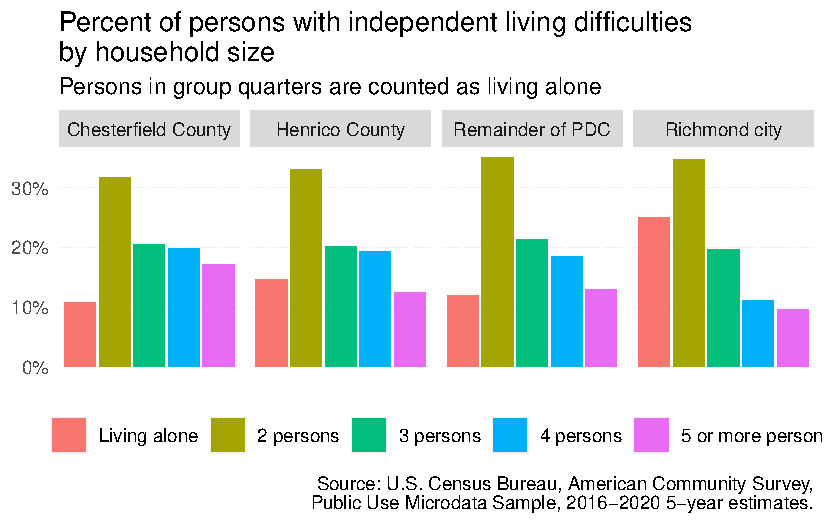
\includegraphics{./part-1-4_files/figure-pdf/fig-ind-liv-size-plot-1.pdf}

}

\caption{\label{fig-ind-liv-size-plot}Percent of persons with
independent living difficulties by household size}

\end{figure}

\hypertarget{veterans-with-disabilities}{%
\section{Veterans with disabilities}\label{veterans-with-disabilities}}

Veterans of military service have access to a range of Department of
Veterans Administration (VA) benefits, including VA home loans. These
benefits also include disability payments for veterans with
service-connected disabilities.

To award disability benefits, the VA assigns each disabled veteran a
\href{https://www.va.gov/disability/about-disability-ratings/}{rating}
from zero to 100 percent based on the severity of their disability or
disabilities. A higher rating reflects more significant impairments, and
accordingly, additional paid benefits to cover lost wages and extra
healthcare services.

From 2016 to 2020, the number of veterans in the region with a
service-connected disability increased by more than 2,800. A significant
majority of this growth occurred among veterans with disability rating
of 70 percent or higher, or those with the most severe physical and/or
mental health challenges.

Despite the increased benefits level associated with the higher rating,
these disabled veterans may be challenged to find accessible and
affordable housing options without additional support.

\begin{figure}

{\centering 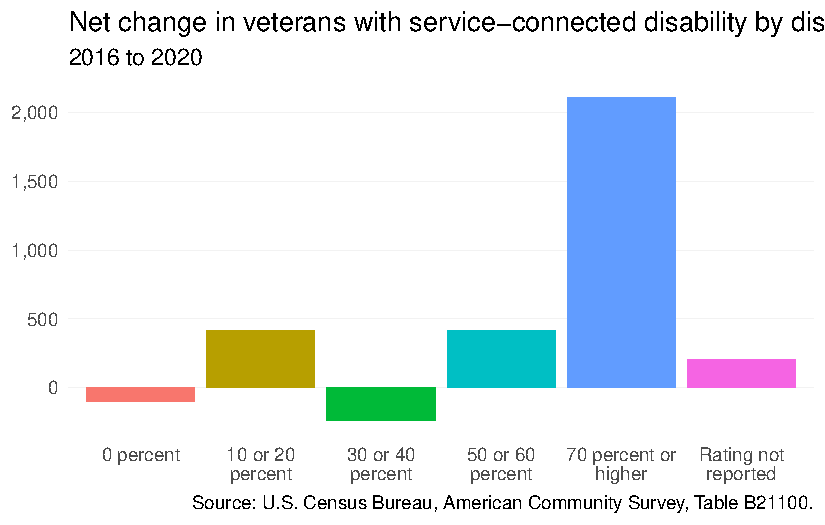
\includegraphics{./part-1-4_files/figure-pdf/fig-vets-plot-1.pdf}

}

\caption{\label{fig-vets-plot}Net change in veterans with
service-connected disability by disability rating}

\end{figure}

\part{PART 2: Housing supply and market changes}

\hypertarget{part-2-1}{%
\chapter{Homeownership}\label{part-2-1}}

\hypertarget{supply}{%
\section{Supply}\label{supply}}

\hypertarget{change-in-stock}{%
\subsection{Change in stock}\label{change-in-stock}}

The stock of homeowner housing has been growing across the region. From
2016 to 2020, owner-occupied housing has increased by 17,436---an
increase of seven percent. Unsurprisingly, much of that growth (93
percent) has occurred in the single-family home market, including
detached and attached homes. The largest share of that single-family
home growth has occurred in Chesterfield County, where there was a net
gain of 7,184 single-family owner-occupied homes.

\begin{figure}

{\centering 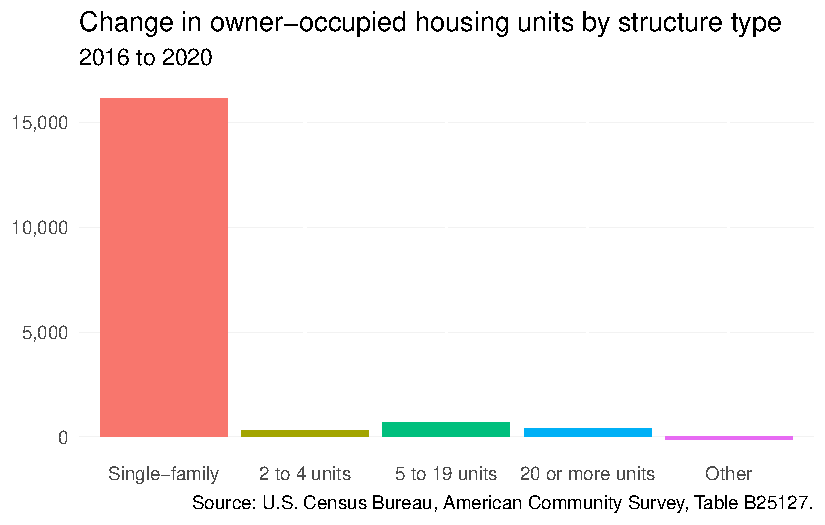
\includegraphics{./part-2-1_files/figure-pdf/oo-structure-plot-1.pdf}

}

\caption{Change in owner-occupied housing units by structure type}

\end{figure}

\hypertarget{age-of-stock}{%
\subsection{Age of stock}\label{age-of-stock}}

Between 2016 and 2020, almost all additions to the homeowner-occupied
housing stock in the region were, intuitively, homes built in the past
decade. However, there have also been thousands of net additions among
homes built before 1940 and between 1980 and 2009. These homes were most
likely previously occupied by renters and have now been reconverted into
homeownership opportunities.

\begin{figure}

{\centering 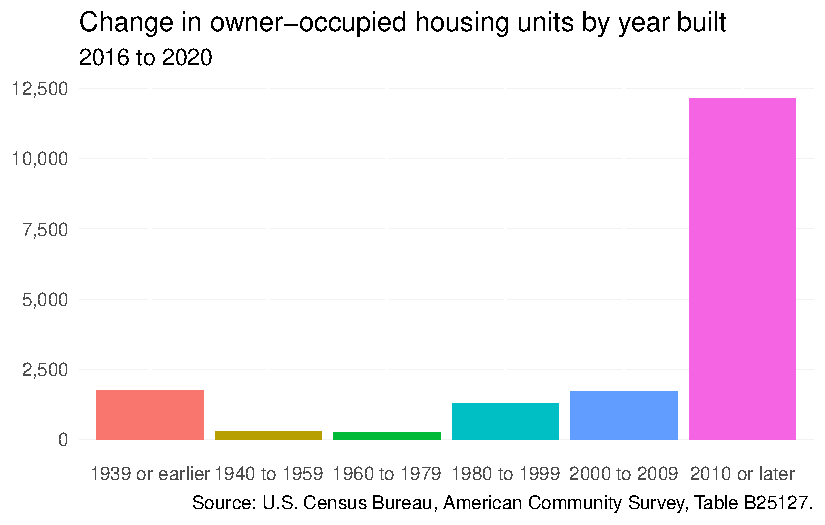
\includegraphics{./part-2-1_files/figure-pdf/oo-age-plot-1.pdf}

}

\caption{Change in owner-occupied housing units by year built}

\end{figure}

\hypertarget{bedrooms}{%
\subsection{Bedrooms}\label{bedrooms}}

The majority of new owner-occupied homes in the region have three or
more bedrooms, continuing design and size trends prevalent since the mid
20th century. At the same time, homeowner households have become
smaller, which creates a surplus of largely unused bedrooms across the
market.

Smaller housing options exist largely in the City of Richmond or Henrico
County. While single-family homes---or condo units---with one- or two-
bedrooms are usually much more affordable, these housing options are
often in older, but highly desirable neighborhoods in the City of
Richmond (i.e., The Fan and Church Hill).

\begin{figure}

{\centering 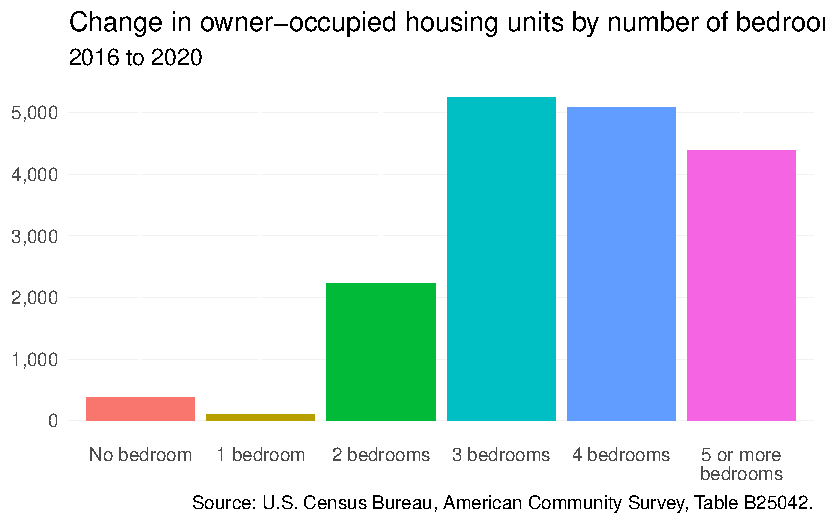
\includegraphics{./part-2-1_files/figure-pdf/oo-beds-plot-1.pdf}

}

\caption{Change in owner-occupied housing units by number of bedrooms}

\end{figure}

\hypertarget{production}{%
\subsection{Production}\label{production}}

All localities in the region experienced single-family construction
declines as a result of the Great Recession from late 2007 to early 2012
--- especially Chesterfield and Henrico. Recovery has been unevenly
distributed, however.

From 2010 onward, every locality has seen increasing single-family home
construction, but the steepest increase has been in Chesterfield County.
From 2010 to 2020, single-family home construction has gone from 545
units to 2,202 per year in a decade --- a 300\% increase. Although
Chesterfield County was on its way to pre-Recession levels, all other
localities are seeing slow growth in the single-family home construction
space.

\begin{figure}

{\centering 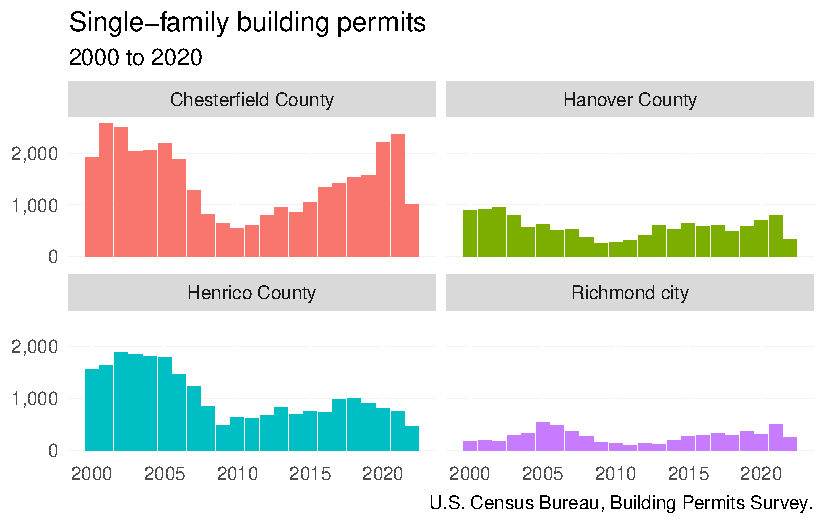
\includegraphics{./part-2-1_files/figure-pdf/bps-plot-1.pdf}

}

\caption{Single-family building permits}

\end{figure}

\hypertarget{homeownership-rate}{%
\section{Homeownership rate}\label{homeownership-rate}}

\hypertarget{by-locality}{%
\subsection{By locality}\label{by-locality}}

Since 2016, overall homeownership rates for localities in the region
have increased slightly. This accounts for the net increase in
homeowners (over 15,000) and relatively steady number of renters over
this time period.

\begin{figure}

{\centering 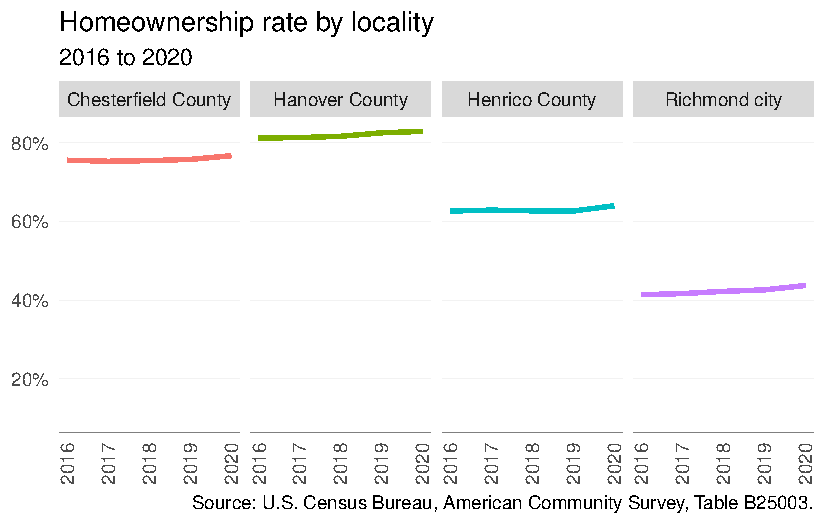
\includegraphics{./part-2-1_files/figure-pdf/ho-rate-plot-1.pdf}

}

\caption{Homeownership rate by locality}

\end{figure}

\hypertarget{by-age-1}{%
\subsection{By age}\label{by-age-1}}

Despite high rents, high debt, and low inventory, younger households
(under 35) have made some progress toward homeownership since 2016.
Their homeownership rate across the region increased from 30 to 35
percent. On the other hand, homeownership rates for middle-age and older
households remained about the same from 2016 to 2020.

\begin{figure}

{\centering 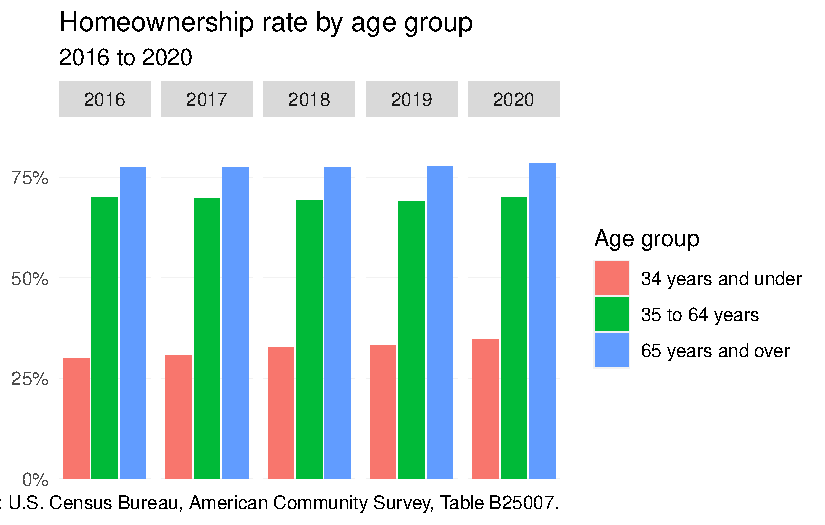
\includegraphics{./part-2-1_files/figure-pdf/ho-age-plot-1.pdf}

}

\caption{Homeownership rate by age group}

\end{figure}

\hypertarget{by-race-and-ethnicity}{%
\subsection{By race and ethnicity}\label{by-race-and-ethnicity}}

Across the region, the homeownership gap remains wide between white
households and households of color. White households in the Richmond
area are the only group with a homeownership rate above 70 percent.
However, several other groups---including Asian, multiracial, and Black
households---have seen slight increases in their homeownership rates
since 2016. At the same time, homeownership rates have fallen slightly
for Hispanic or Latino households and those of another race.

\begin{figure}

{\centering 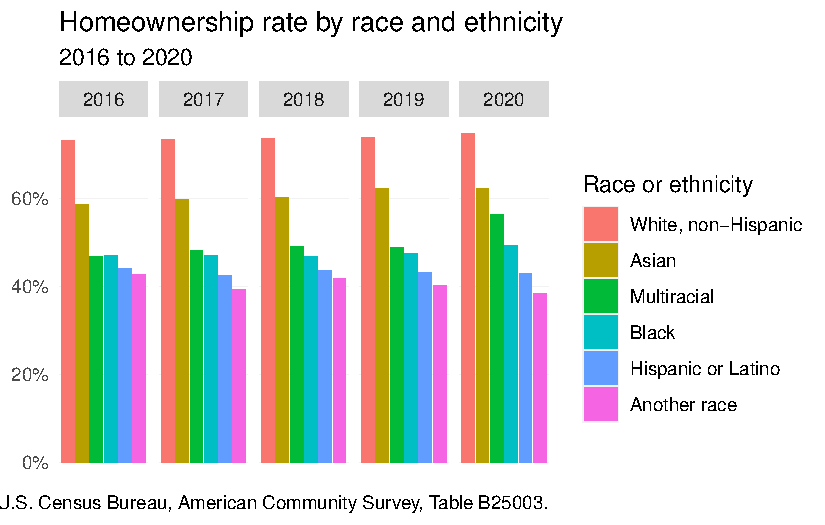
\includegraphics{./part-2-1_files/figure-pdf/ho-race-plot-1.pdf}

}

\caption{Homeownership rate by race and ethnicity}

\end{figure}

\hypertarget{for-sale-market}{%
\section{For-sale market}\label{for-sale-market}}

\hypertarget{closed-sales}{%
\subsection{Closed sales}\label{closed-sales}}

Home sales in the region continued to follow seasonal patterns during
the COVID-19 pandemic. All localities saw reductions in typical sales
volumes during early parts of the pandemic (spring to early summer
2020)---no doubt a result of stay-at-home orders. But by 2021, sales
volume began to climb back as historically low interest rates
incentivized home buying.

\begin{figure}

{\centering 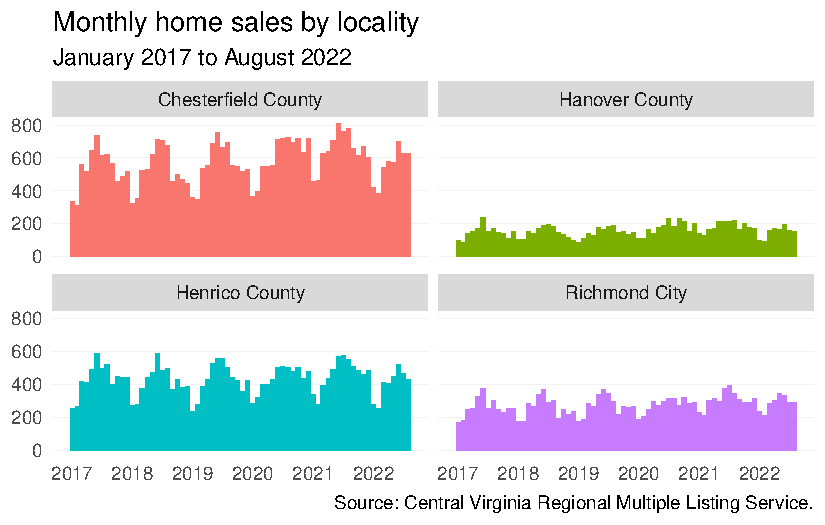
\includegraphics{./part-2-1_files/figure-pdf/sales-plot-1.pdf}

}

\caption{Monthly home sales by locality}

\end{figure}

Chesterfield County continued to lead the region in home sales---hitting
a monthly peak in June 2021, with a total of 809 sales. In nearly all
localities except for Chesterfield County, the average monthly home
sales has largely remained the same. Only in Chesterfield County was
there a more than 10 percent increase in average monthly home sales
between 2019 and 2021.

\begin{figure}

{\centering 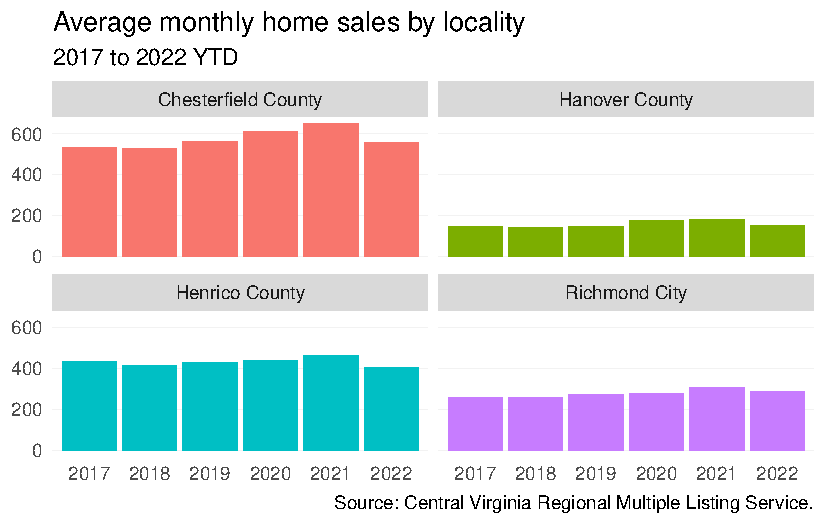
\includegraphics{./part-2-1_files/figure-pdf/sales-avg-plot-1.pdf}

}

\caption{Average monthly home sales by locality}

\end{figure}

\hypertarget{sales-price}{%
\subsection{Sales price}\label{sales-price}}

Median home prices have continued to climb in the Richmond
Region---reaching over \$300,000 in all four major localities. The
greatest price increases have occurred in the City of Richmond during
2022, where the median home price went from \$303,941 in February to
\$389,950 in June, a 28 percent increase. Home prices are continuing to
trend upward in spite of rising mortgage interest rates.

Hanover County remains the most expensive locality in the region with a
median home price of \$464,000 in July 2022, followed by the
Chesterfield County (\$378,671), Henrico County (\$370,000), and the
City of Richmond (\$352,500).

\begin{figure}

{\centering 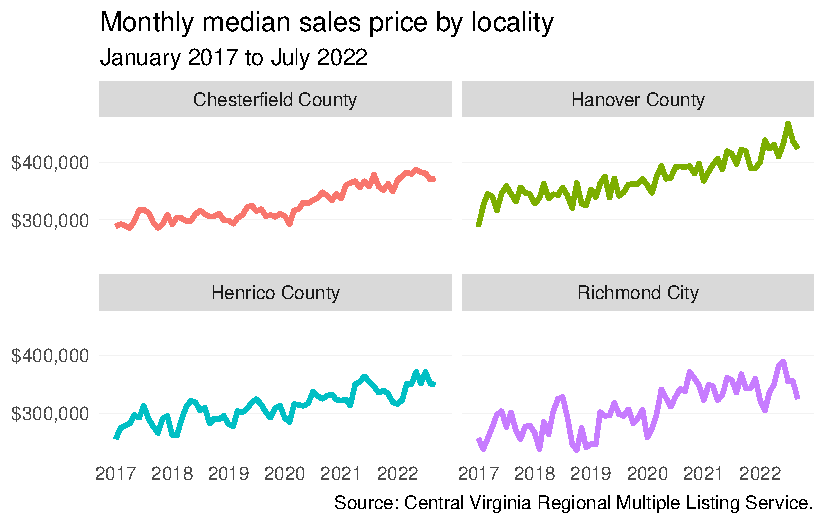
\includegraphics{./part-2-1_files/figure-pdf/sales-price-plot-1.pdf}

}

\caption{Monthly median sales price by locality}

\end{figure}

\hypertarget{supply-1}{%
\subsection{Supply}\label{supply-1}}

The inventory of for-sale housing before the pandemic typically sat at
two months or more---meaning that it would take two or more months to
sell at current prices. A healthy level of supply has said to be five or
six months worth, but in recent years the region has been below that,
which indicates a strong seller's market.

When pandemic began in March 2020, months supply dropped to two months
and then by June 2020 hit a low of one month and has sat squarely there
ever since. Even amid rising interest rates in 2022 and talks of a
housing slump, months supply continues to remain low.

\begin{figure}

{\centering 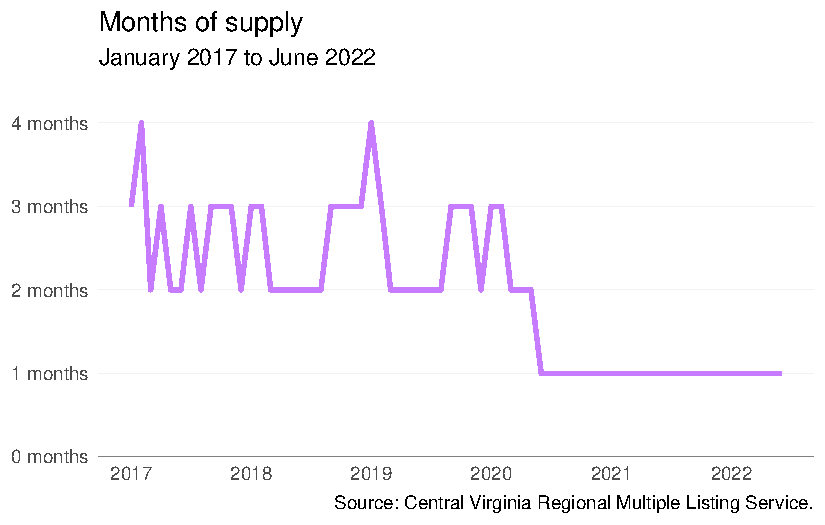
\includegraphics{./part-2-1_files/figure-pdf/supply-plot-1.pdf}

}

\caption{Months of supply}

\end{figure}

\hypertarget{starter-homes}{%
\subsection{Starter homes}\label{starter-homes}}

Starter homes provide young adults the ability to get on the first rung
of the homeownership ladder. This allows many young adults the ability
to build equity before their household grows (i.e.~marriage and
children). But starter homes are becoming more and more scarce. This has
largely because those starter home opportunities are not coming to
market. In some cases, older homes occupied by seniors are not hitting
the market because senior desire to age-in-place remains high or seniors
simply cannot find other affordable options themselves. Starter homes
are also ripe for investor flipping, which leaves first-time homebuyers
competing with all cash offers.

In addition, smaller homes do not make up a significant share of new
construction stock. Smaller homes (two-bedroom or less) are often more
desirable among seniors and young adults without children. The lack of
this stock prevents the movement of households from different rungs
along the homeownership ladder --- locking homeowners into homes that
often no longer work for them.

In 2021, the Virginia REALTORS® (VAR) conducted an analysis of the
number and share of starter homes sold in Virginia from 2013 to
mid-2021. This analysis was included in the statewide housing study
conducted by HousingForward Virginia as part of HB 854. To calculate the
number and share of starter homes sold, VAR calculated the number of
homes sold that would be affordable to a household making 80 percent of
AMI.

For the region, the share of starter homes sold has been in a steady
decline. The greatest decrease has occurred in Chesterfield County,
where the share of starter homes sold has gone from 63 percent to 46
percent. The smallest decreased occurred in Henrico County, a decrease
of only 8 percentage points.

\begin{figure}

{\centering 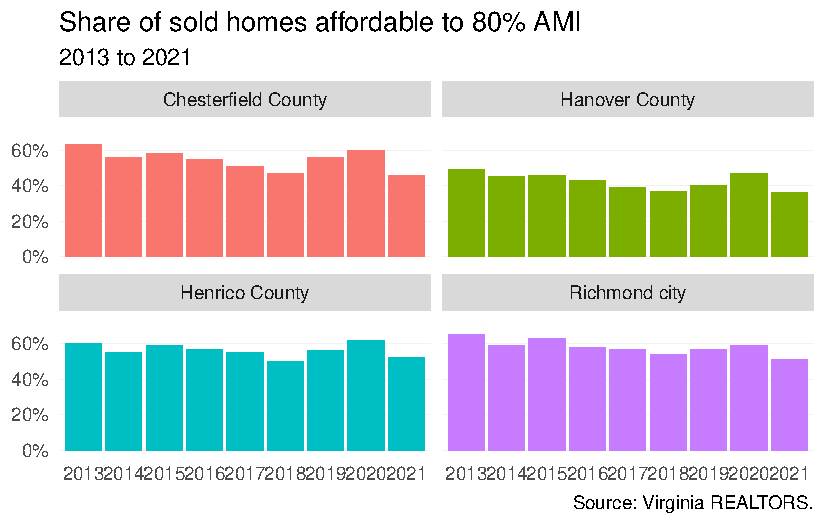
\includegraphics{./part-2-1_files/figure-pdf/starter-plot-1.pdf}

}

\caption{Share of sold homes affordable to 80\% AMI}

\end{figure}

\hypertarget{new-construction-versus-resale}{%
\section{New construction versus
resale}\label{new-construction-versus-resale}}

\hypertarget{sales-price-1}{%
\subsection{Sales price}\label{sales-price-1}}

The affordability of resale homes compared to new construction has often
made them the first rung on the homeownership ladder. But since the
start of the pandemic, the median resale home price has risen above the
\$300,000 mark and in June 2022 reached a high of \$371,250.

During this timeframe, new construction median home prices have remained
above \$350,000 and throughout 2022 so far have stayed above \$400,000.
On average, there is a \$89,127 difference between new construction and
resale sales price---leaving new construction significantly out of reach
for lower income households.

\begin{figure}

{\centering 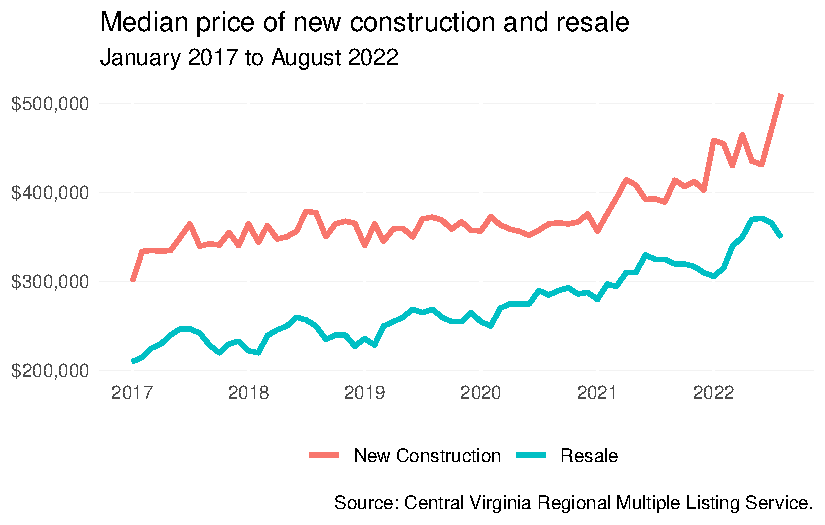
\includegraphics{./part-2-1_files/figure-pdf/comp-price-plot-1.pdf}

}

\caption{Median price of new construction and resale}

\end{figure}

\hypertarget{bedrooms-1}{%
\subsection{Bedrooms}\label{bedrooms-1}}

The majority of home sales in the region have been for three- and
four-bedroom homes --- roughly three in four homes sold in the past five
years. Nuances exist at either end of the bedroom spectrum.

New construction of homes with one- to two-bedrooms has been increasing
--- going from six percent of sales in 2017 to nine percent in 2022 YTD.
At the other end, new construction of five or more bedroom homes has
increased as well with an increase of three percent (15 percent of sales
in 2017 to 18 percent in 2022 YTD). For resale homes, the share of homes
by bedroom has remained largely unchanged each year.

\begin{figure}

{\centering 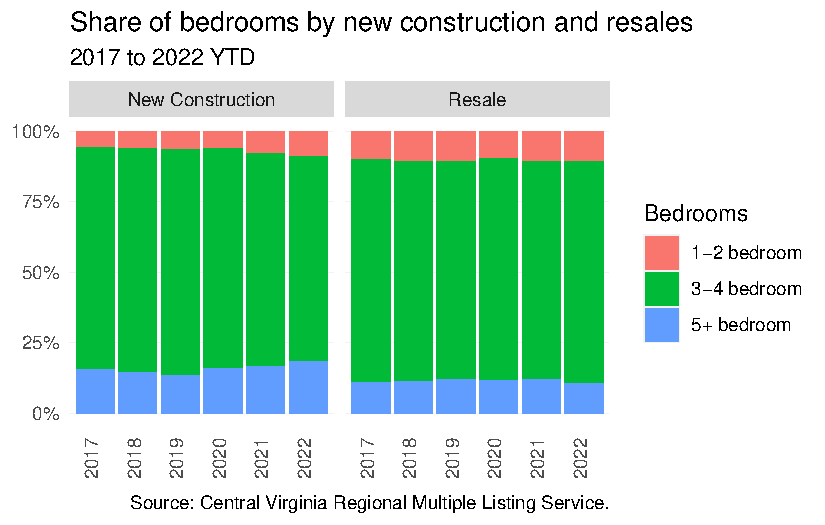
\includegraphics{./part-2-1_files/figure-pdf/comp-br-plot-1.pdf}

}

\caption{Share of bedrooms by new construction and resales}

\end{figure}

\hypertarget{size}{%
\subsection{Size}\label{size}}

In the past five years, there have been clear differences in new
construction and resale sales by square footage. The majority of resale
homes have been under 2,000 square feet, while new construction is
overwhelmingly over 2,000 square feet. These differences have clear
implications on home prices (i.e.~more square footage means higher
prices). But across the region, minimum requirements set out by
localities in zoning ordinances impact these builder decisions.

Building smaller homes is less profitable given the rising cost to
develop a single detached home (e.g.~rising land, infrastructure, and
regulatory costs). In order to maximize profit, home builders need to
increase square footage to recoup costs and meet development
requirements.

\begin{figure}

{\centering 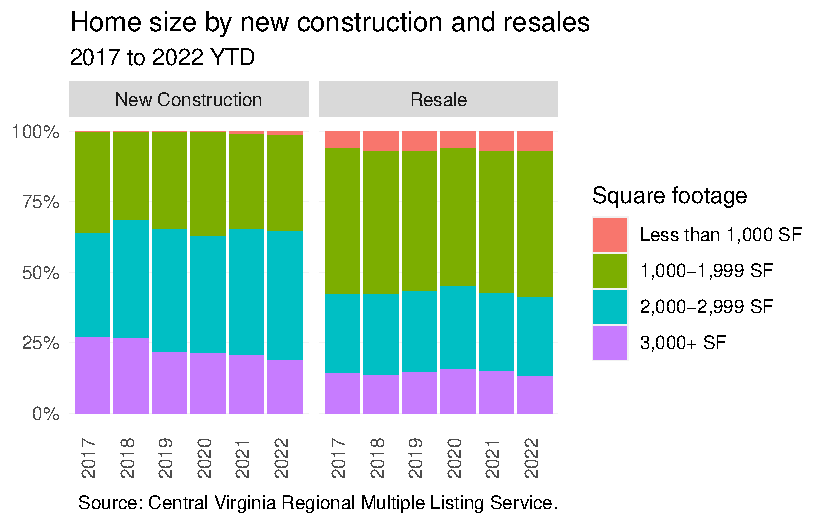
\includegraphics{./part-2-1_files/figure-pdf/comp-sf-plot-1.pdf}

}

\caption{Home size by new construction and resales}

\end{figure}

\hypertarget{part-2-2}{%
\chapter{Rental homes}\label{part-2-2}}

\hypertarget{supply-2}{%
\section{Supply}\label{supply-2}}

\hypertarget{change-in-stock-1}{%
\subsection{Change in stock}\label{change-in-stock-1}}

While many renters across the region do live in multifamily buildings
(with 5 or more units), the second largest share of rental housing is
single-family housing (either attached or detached). In 2020, over a
third (37 percent) of rental housing in the region consisted of
single-family housing, while 49 percent was located in buildings with 5
or more units. There has been little change in these percentages since
2016.

Changes in the shares of rental housing have been small --- but those
changes have been among rental housing with 20 or more units (17 percent
in 2016 to 19 percent in 2020) and 2 to 4 unit buildings (14 percent in
2016 down to 13 percent in 2020).

\begin{figure}

{\centering 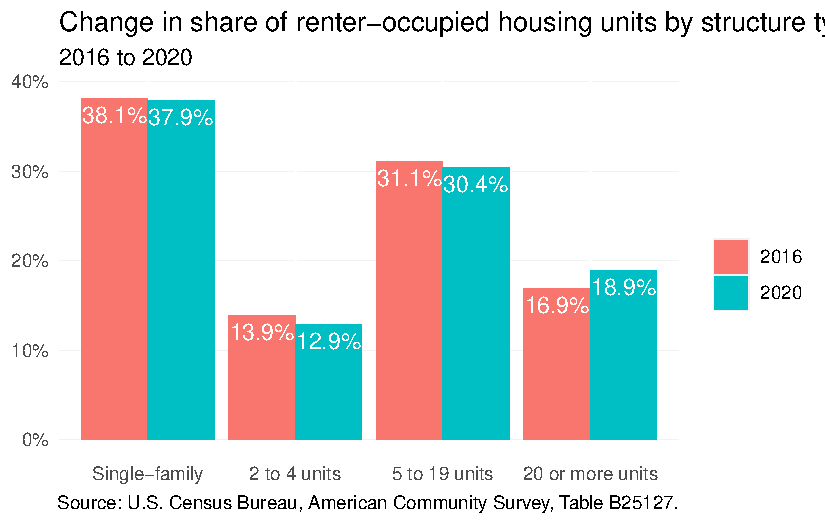
\includegraphics{./part-2-2_files/figure-pdf/fig-ro-structure-percent-1.pdf}

}

\caption{\label{fig-ro-structure-percent}Change in share of
renter-occupied housing units by structure type}

\end{figure}

The raw changes in rental housing were most felt in Henrico County and
the City of Richmond. In Henrico, there was a 1,930 increase in
single-family rental housing and a 1,357 decrease in 2 to 4 unit rental
housing (i.e.~duplexes, triplexes, and quads).

The City of Richmond saw a contrasting decrease in single-family rentals
(-1,921), while also experiencing a 2,134 increase in rental housing
located in buildings with 20 or more units. Chesterfield County has seen
slight increases in multifamily housing of all types, while Hanover
County has not seen much change at all.

\begin{figure}

{\centering 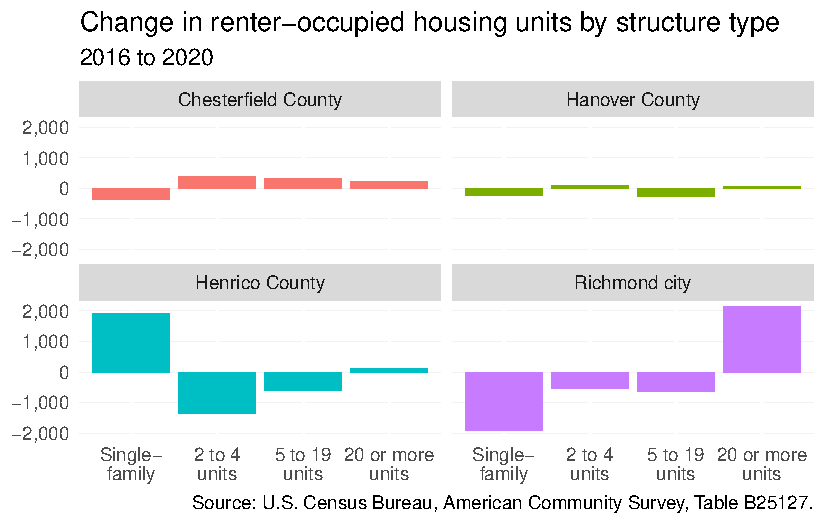
\includegraphics{./part-2-2_files/figure-pdf/fig-ro-structure-1.pdf}

}

\caption{\label{fig-ro-structure}Change in renter-occupied housing units
by structure type}

\end{figure}

\hypertarget{age-of-stock-1}{%
\subsection{Age of stock}\label{age-of-stock-1}}

Since 2016, the region has seen major changes in the age of its rental
stock as existing homes transition from being owned to leased out, or
vice-versa. Of note, every locality except for Hanover saw significant
increases in the number of renter-occupied homes built between 1980 and
1999.

These homes---now over 20 years old---are likely becoming the target of
investors purchasing from homeowners, making certain improvements, and
renting them out. In Henrico County, this trend was even more prevalent
among homes built between 1960 and 1979.

Conversely, Chesterfield and Henrico each had over 1,000 homes built
between 2000 and 2009 change from renter- to owner-occupied. The largest
losses in rental stock, however, occurred in Richmond among homes built
prior to 1980. Several factors could explain this decline:

\begin{itemize}
\tightlist
\item
  Actual demolition of very old, low-quality homes,
\item
  Duplexes and triplexes converted into single-family homes, and
\item
  Single-family rentals purchased by buyers who now live in the home.
\end{itemize}

\begin{figure}

{\centering 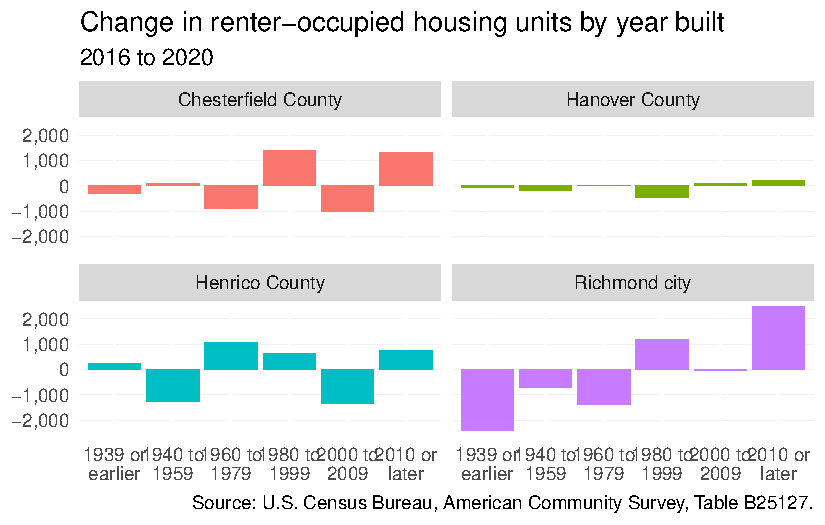
\includegraphics{./part-2-2_files/figure-pdf/fig-ro-year-built-1.pdf}

}

\caption{\label{fig-ro-year-built}Change in renter-occupied housing
units by year built}

\end{figure}

\hypertarget{bedrooms-2}{%
\subsection{Bedrooms}\label{bedrooms-2}}

Rental homes in the Richmond region are most likely to have one or two
bedrooms. While the number of one-bedroom apartments has continued to
increase (+1,617) from 2016, the number of two-bedroom units has
decreased by 2,500.

The increasing supply of one-bedroom apartments coincides with a similar
increase in studio apartments---these unit sizes reflect new apartments,
largely in Richmond, marketed for college students and other young
adults.

The dwindling number of two-bedroom rental homes may reflect small
single-family rentals in older neighborhoods transitioning to
owner-occupancy, as there is a similar (but much less significant)
decline in three-bedroom units.

\begin{figure}

{\centering 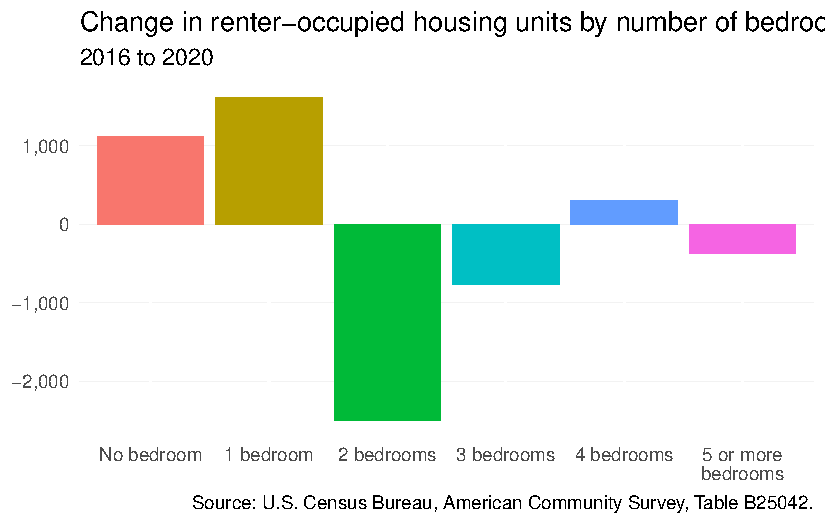
\includegraphics{./part-2-2_files/figure-pdf/fig-ro-bedrooms-1.pdf}

}

\caption{\label{fig-ro-bedrooms}Change in renter-occupied housing units
by number of bedrooms}

\end{figure}

\hypertarget{production-1}{%
\subsection{Production}\label{production-1}}

Construction of multifamily properties (with 5 units or more) has been
sporadic since the end of the Great Recession. In all localities aside
from Hanover County, there have been waves and dips in the multifamily
building construction. Hanover has seen little to no activity throughout
the last two decades, while Chesterfield County and Richmond have seen
the bulk of activity.

During the latter half of the last decade, Chesterfield County had a
boom in multifamily construction --- nearing 1,500 units in 2019.
Meanwhile, Richmond's multifamily construction saw dips following the
Great Recession and again in 2018, but has largely been up in the last
couple years of the 2010s. Although Henrico County had dips in 2016 and
2018, multifamily construction has more often than not been above the
700 unit mark.

\begin{figure}

{\centering 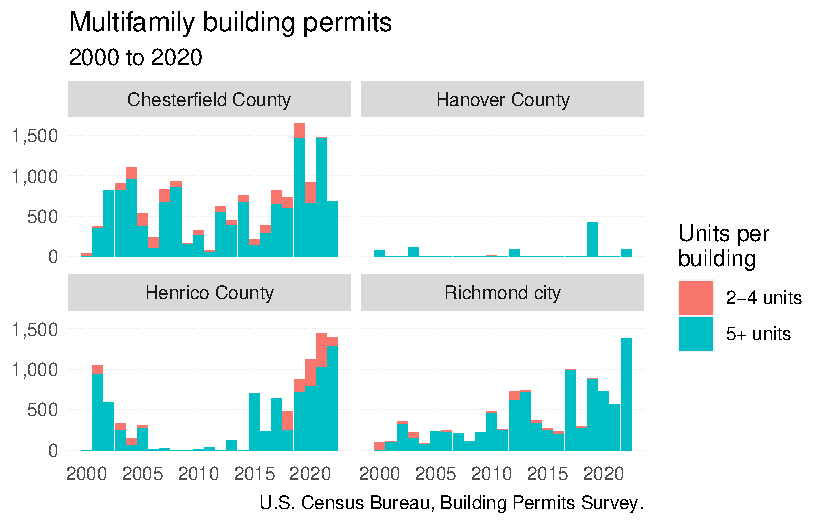
\includegraphics{./part-2-2_files/figure-pdf/fig-mf-permits-1.pdf}

}

\caption{\label{fig-mf-permits}Multifamily building permits}

\end{figure}

\hypertarget{rental-market}{%
\section{Rental market}\label{rental-market}}

\hypertarget{average-market-asking-rent}{%
\subsection{Average market asking
rent}\label{average-market-asking-rent}}

Rental demand reached a fever pitch amid the ongoing COVID-19 pandemic.
With eviction moratoriums and a flow of rental assistance, low supply
gave way to historic rent increases. The average market asking rent in
the region reached a two-decade high of \$1,395 in the first quarter of
2022.

\begin{figure}

{\centering 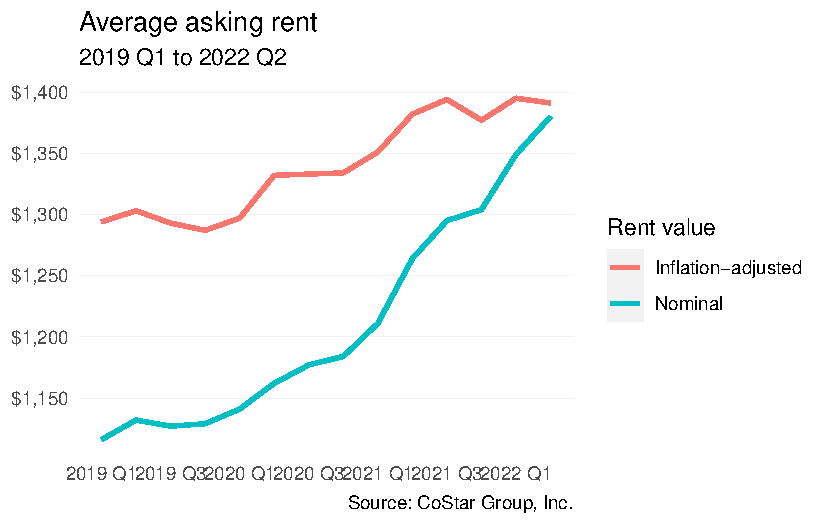
\includegraphics{./part-2-2_files/figure-pdf/fig-avg-rent-1.pdf}

}

\caption{\label{fig-avg-rent}Average asking rent}

\end{figure}

Large quarterly increases in average rents began in early 2021 and have
continued to the present. From the first to second quarters of this
year, rents increased by \$31. However, this relative growth was very
near the change in inflation over that same period.

\begin{figure}

{\centering 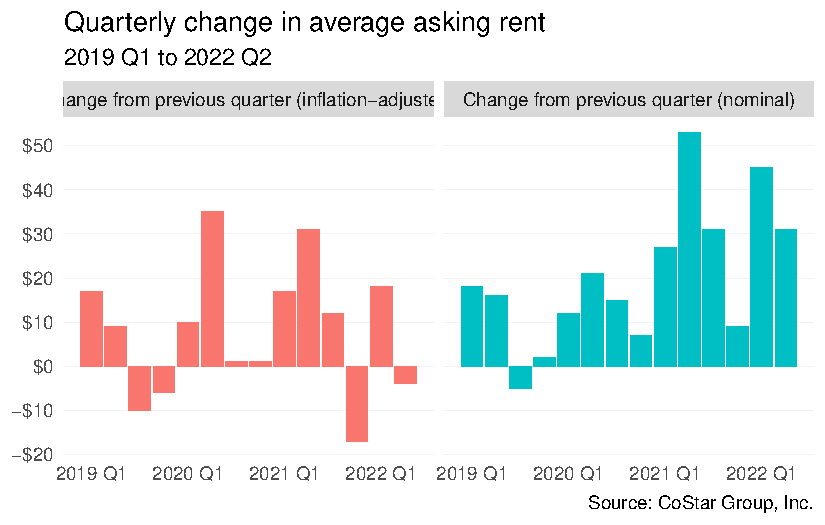
\includegraphics{./part-2-2_files/figure-pdf/fig-avg-rent-change-1.pdf}

}

\caption{\label{fig-avg-rent-change}Quarterly change in average asking
rent}

\end{figure}

\hypertarget{rents-by-submarket}{%
\subsection{Rents by submarket}\label{rents-by-submarket}}

Although not adjusted for inflation, rents by submarket show that there
are distinct average rents across the region. Since 2010, the steepest
increases have occurred in the counties. Northside Richmond remains the
least expensive submarket with an average rent of \$1,037 in the second
quarter of this year, while Midlothian is the most expensive at \$1,655.

\begin{figure}

{\centering 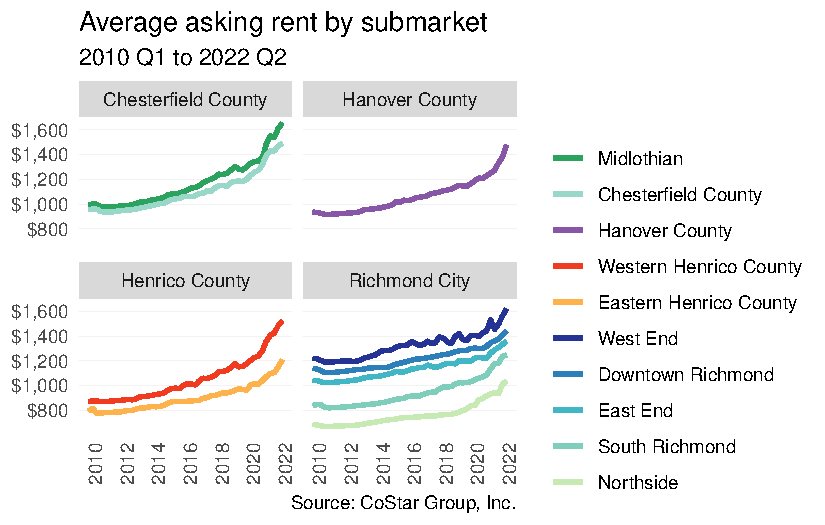
\includegraphics{./part-2-2_files/figure-pdf/fig-avg-rent-submarket-1.pdf}

}

\caption{\label{fig-avg-rent-submarket}Average asking rent by submarket}

\end{figure}

\hypertarget{rents-by-bedrooms}{%
\subsection{Rents by bedrooms}\label{rents-by-bedrooms}}

Rents in the region have risen the most among three-bedroom and
two-bedroom apartments, reflecting continued demand for units that have
actually \emph{declined} in supply since 2016. In contrast, average
rents for studio and one-bedroom apartments---which grew by more than
2,700 units since 2016---have increased less than \$100 over the last
decade when adjusted for inflation.

\begin{figure}

{\centering 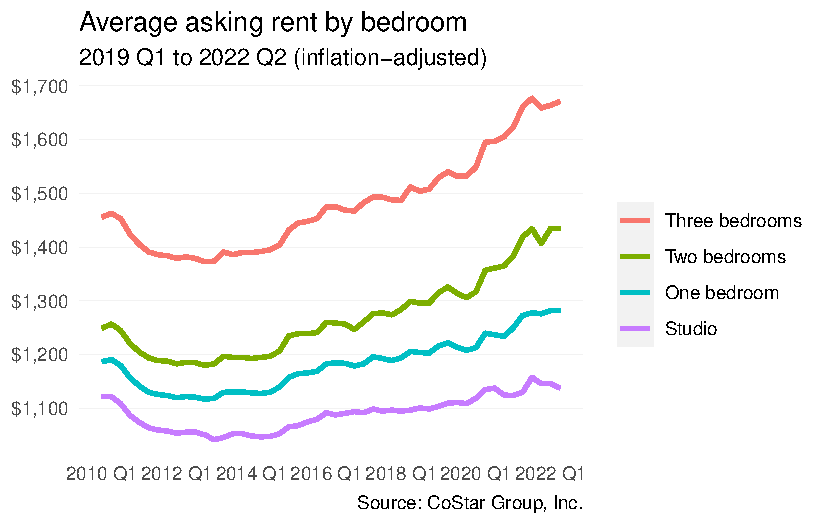
\includegraphics{./part-2-2_files/figure-pdf/fig-avg-rent-br-1.pdf}

}

\caption{\label{fig-avg-rent-br}Average asking rent by bedroom}

\end{figure}

\hypertarget{rents-by-age-of-units}{%
\subsection{Rents by age of units}\label{rents-by-age-of-units}}

Recently constructed rental housing (built in 2010 and after) leads
average asking rents at \$1,614. As expected, rental costs correlate to
the period in which they were built --- with older rental housing being
less expensive. Pre-1980 rental housing is roughly \$400 cheaper than
more recent rental housing.

In the last decade, more recent rental housing had steady and modest
increases; only increasing \$80 from Q1 2012 to Q2 2022. But older
rental housing had much more dramatic increases; increasing an average
of \$257 in that same time period.

Rental housing built between 1980 and 2009 had especially steep
increases during the height of the pandemic (Q1 2020 to Q3 2021). In
this time, the average asking rent increased by over \$130, while rent
increases for newer rental housing and pre-1980 housing increased by
less than \$100.

\begin{figure}

{\centering 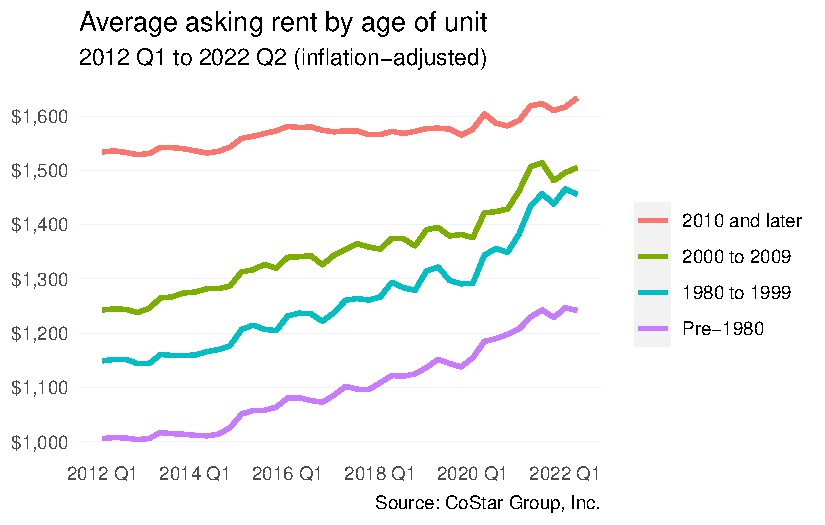
\includegraphics{./part-2-2_files/figure-pdf/fig-rents-built-1.pdf}

}

\caption{\label{fig-rents-built}Average asking rent by age of unit}

\end{figure}

\hypertarget{rental-vacancy}{%
\section{Rental vacancy}\label{rental-vacancy}}

For much of the past two decades, vacancy rates have fluctuated
seasonally as new people enter and leave the rental housing market.
Across the region, submarkets have largely had vacancy rates below ten
percent. In 2022, the regional average vacancy rate to-date was five
percent.

However, some submarkets in the region have lower than average vacancy
rates; Hanover County (1 percent), Eastern Henrico (3 percent),
Northside (3 percent), and East End (4 percent) have significantly lower
vacancy rates.

\begin{figure}

{\centering 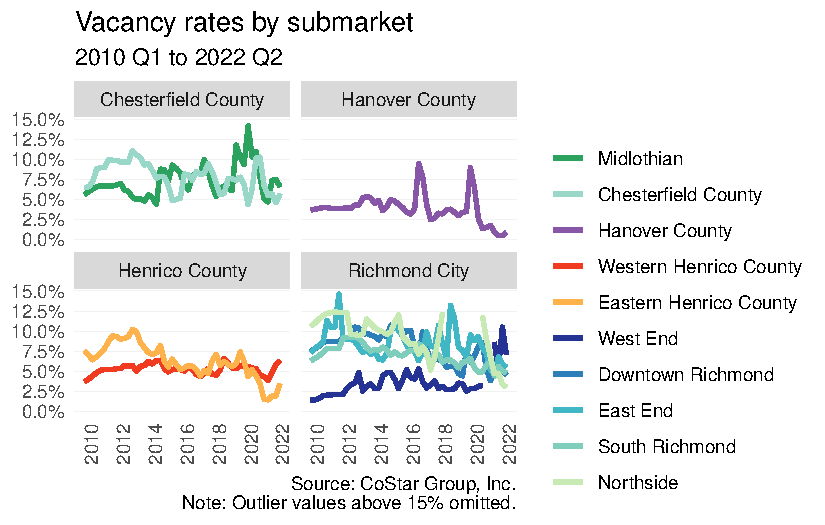
\includegraphics{./part-2-2_files/figure-pdf/fig-vacancy-1.pdf}

}

\caption{\label{fig-vacancy}Vacancy rates by submarket}

\end{figure}

\hypertarget{part-2-3}{%
\chapter{Housing assistance}\label{part-2-3}}

This chapter covers the range of housing assistance in the region
supported by federal, state, and local programs.

\hypertarget{affordable-rental-housing}{%
\section{Affordable rental housing}\label{affordable-rental-housing}}

An array of federal housing assistance programs help low-income
residents across the region with rental housing opportunities. Today,
there are approximately 25,969 dedicated affordable rental homes found
across 240 properties in the Richmond area. These include units both
currently occupied and in development.

\begin{tcolorbox}[enhanced jigsaw, colback=white, colbacktitle=quarto-callout-tip-color!10!white, bottomrule=.15mm, opacitybacktitle=0.6, colframe=quarto-callout-tip-color-frame, breakable, opacityback=0, bottomtitle=1mm, titlerule=0mm, coltitle=black, leftrule=.75mm, left=2mm, title=\textcolor{quarto-callout-tip-color}{\faLightbulb}\hspace{0.5em}{Tip}, toptitle=1mm, arc=.35mm, rightrule=.15mm, toprule=.15mm]
In the Richmond region, many affordable rental properties also receive
assistance from the Virginia Housing Trust Fund, as well as local
sources such as CDBG and HOME grants. The City of Richmond also awards
funding to affordable rental projects with its own trust fund.
\end{tcolorbox}

\hypertarget{subsidy-types}{%
\subsection{Subsidy types}\label{subsidy-types}}

Over half (51 percent) of all affordable rental homes in the region rely
\emph{solely} on the LIHTC program. Another 31 percent have layered
multiple subsidies together, reflecting the capital and funding
requirements needed to develop new affordable housing.

The other significant source of dedicated affordable housing continues
to be more than 3,600 Public Housing units managed by Richmond
Redevelopment and Housing Authority.

\begin{tcolorbox}[enhanced jigsaw, colback=white, colbacktitle=quarto-callout-note-color!10!white, bottomrule=.15mm, opacitybacktitle=0.6, colframe=quarto-callout-note-color-frame, breakable, opacityback=0, bottomtitle=1mm, titlerule=0mm, coltitle=black, leftrule=.75mm, left=2mm, title=\textcolor{quarto-callout-note-color}{\faInfo}\hspace{0.5em}{Note}, toptitle=1mm, arc=.35mm, rightrule=.15mm, toprule=.15mm]
Descriptions of each rental assistance program are available on the
\href{https://preservationdatabase.org/documentation/program-descriptions/}{NHPD
website}.
\end{tcolorbox}

\begin{figure}

{\centering 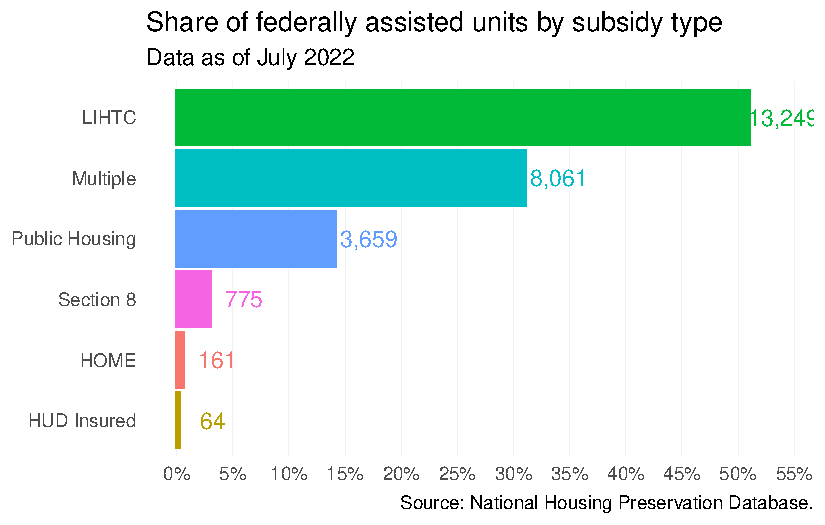
\includegraphics{./part-2-3_files/figure-pdf/fig-subsidy-overall-1.pdf}

}

\caption{\label{fig-subsidy-overall}Share of federally assisted units by
subsidy}

\end{figure}

\hypertarget{layered-subsidies}{%
\subsection{Layered subsidies}\label{layered-subsidies}}

In an effort to maximize assistance, rental subsidy programs are often
layered together into single projects. Among the 8,061 units with
multiple subsidies, over half have either a 4\% or 9\% LIHTC tax
credit---or both ``twinned'' together. Section 8 Housing Finance and
Development Agency (HFDA) New Construction and Loan Management Set-Aside
(LMSA) programs are also common types.

``Other'' subsidies generally include HUD insurance programs and other,
less common, Section 8 programs. Still, these minor assistance packages
nevertheless provide helping subsidy to almost three-in-four units with
multiple affordability contracts.

\hypertarget{tbl-multiple}{}
\begin{table}
\caption{\label{tbl-multiple}Active subsidies in units with mutiple subsidies }\tabularnewline

\centering
\begin{tabular}{l|r|r}
\hline
Detailed subsidy type & Units with subsidy & Percent of total\\
\hline
LIHTC 4\% Tax Credit & 4,747 & 58.9\%\\
\hline
LIHTC 9\% Tax Credit & 4,371 & 54.2\%\\
\hline
Section 8 HFDA/8 NC & 1,584 & 19.7\%\\
\hline
Section 8 LMSA & 1,173 & 14.6\%\\
\hline
Other & 5,880 & 72.9\%\\
\hline
\multicolumn{3}{l}{\rule{0pt}{1em}makecell[l]{Note: Totals do not add to 100\% because units are percent of all 8,061 units with multiple subsidies. \ Sources: National Housing Preservation Database and Virginia Housing.}}\\
\end{tabular}
\end{table}

\hypertarget{locations}{%
\subsection{Locations}\label{locations}}

The map below shows the locations of affordable rental properties in the
Richmond region. Each color corresponds to the property's subsidy as
recorded in the National Housing Preservation Database, or if multiple
subsidies are currently active.

\begin{figure}

{\centering \includegraphics{./part-2-3_files/figure-pdf/fig-nhpd-map-1.pdf}

}

\caption{\label{fig-nhpd-map}Federally-assisted rental housing
properties}

\end{figure}

Richmond continues to support the majority of affordable rentals in the
region (about 60 percent---more than 15,200). While Chesterfield and
Henrico counties both have similar amounts of LIHTC-only units, Henrico
has nearly 2,900 additional units supported by multiple
subsidies---generally combinations of LIHTC and a Section 8 program.

\begin{figure}

{\centering \includegraphics{./part-2-3_files/figure-pdf/fig-subsidy-location-1.pdf}

}

\caption{\label{fig-subsidy-location}Federally assisted units by subsidy
and locality}

\end{figure}

\hypertarget{changes-since-2020}{%
\subsection{Changes since 2020}\label{changes-since-2020}}

Since January 2020, the region has seen 57 new rental subsidies added,
which increased the number of active affordability contracts on units by
4,393. Over that same period, 17 subsidies ended, affecting 1,633 units.
Some properties had multiple subsidies either added or expired. In all,
there was a net addition of 2,760 rental affordability contracts.

\hypertarget{tbl-change}{}
\begin{table}
\caption{\label{tbl-change}Added and removed affordable rental contracts since 2020 }\tabularnewline

\centering
\begin{tabular}{l|r|r|r}
\hline
 & Subsidies & Properties affected & Units included\\
\hline
Added & 57 & 53 & 4,393\\
\hline
Removed & -17 & -16 & -1,633\\
\hline
\textbf{Net change} & \textbf{40} & \textbf{37} & \textbf{2,760}\\
\hline
\multicolumn{4}{l}{\rule{0pt}{1em}Sources: National Housing Preservation Database and Virginia Housing.}\\
\end{tabular}
\end{table}

New LIHTC units (net 2,129) comprised the majority of added affordable
rentals, followed by Section 8 contracts (net 1,132). Net losses of
affordable rental contracts occurred in projects supported by HOME
funding and HUD insurance.

\begin{figure}

{\centering \includegraphics{./part-2-3_files/figure-pdf/fig-change-1.pdf}

}

\caption{\label{fig-change}Additions and removals of subsidized rental
units}

\end{figure}

While LIHTC additions drove new affordable supply in Richmond and
Chesterfield, new (or renewed) Section 8 contracts covered more than 400
units in Henrico. Over 500 units in Richmond and Henrico saw HUD
insurance contracts expire; however, many of these are in projects with
another form of rental assistance that has not expired.

\begin{figure}

{\centering \includegraphics{./part-2-3_files/figure-pdf/fig-change-locality-1.pdf}

}

\caption{\label{fig-change-locality}Net change in subsidized rental unit
contracts by locality}

\end{figure}

\hypertarget{lihtc-preservation}{%
\subsection{LIHTC preservation}\label{lihtc-preservation}}

LIHTC properties have a 30 year commitment to affordability, but only a
15 year compliance period, wherein property owners can increase rents.
Nonprofit developers will often seek new allocation of tax credits
before their commitment period ends, but there is often little incentive
for for-profit developers to maintain affordability restrictions past
the compliance period.

By 2040, a large portion of active LIHTC units will be outside the 30
year commitment period --- even far more will be outside the 15 year
compliance period. Just over 13,000 LIHTC units will be beyond the 30
year commitment period by 2040, which accounts for well over half of all
active LIHTC units as of early 2022.

\begin{figure}

{\centering \includegraphics{./part-2-3_files/figure-pdf/fig-lihtc-1.pdf}

}

\caption{\label{fig-lihtc}Percent of active LIHTC units by end of
commitment period}

\end{figure}

\hypertarget{public-housing}{%
\subsection{Public Housing}\label{public-housing}}

The redevelopment of public housing in the City of Richmond has begun to
take shape at the first of the ``Big Six'' public housing courts ---
\textbf{Creighton Court}. This public housing property located in
Richmond's far East End consisted of 504 public housing units.

As part of their first phase of redevelopment, RRHA has begun demolition
of Creighton Court, with plans to develop roughly 700 units of
mixed-income housing. Construction on Phase 1 is expected to begin in
Winter 2022 with the entire redevelopment process expected to last ten
years.

RRHA's next focus area will be \textbf{Gilpin Court}, north of Jackson
Ward, where about 780 public housing units reside. In November 2021,
RRHA and the City of Richmond were awarded a Choice Neighborhoods
Planning Grant by the U.S. Department of Housing and Urban Development
for \$450,000.

This planning grant is being utilized to facilitate the community
planning process around not only Gilpin Court, but the Jackson Ward
community --- including strategies to undo the negative impacts of
interstate development on the historically Black communities of Jackson
Ward and North Jackson Ward.

\begin{longtable}[]{@{}
  >{\raggedright\arraybackslash}p{(\columnwidth - 6\tabcolsep) * \real{0.3562}}
  >{\raggedleft\arraybackslash}p{(\columnwidth - 6\tabcolsep) * \real{0.2192}}
  >{\raggedleft\arraybackslash}p{(\columnwidth - 6\tabcolsep) * \real{0.2603}}
  >{\raggedleft\arraybackslash}p{(\columnwidth - 6\tabcolsep) * \real{0.1644}}@{}}
\caption{Net change in units for public housing
redevelopment}\tabularnewline
\toprule()
\begin{minipage}[b]{\linewidth}\raggedright
Public housing community
\end{minipage} & \begin{minipage}[b]{\linewidth}\raggedleft
Original units
\end{minipage} & \begin{minipage}[b]{\linewidth}\raggedleft
Replacement units
\end{minipage} & \begin{minipage}[b]{\linewidth}\raggedleft
Net change
\end{minipage} \\
\midrule()
\endfirsthead
\toprule()
\begin{minipage}[b]{\linewidth}\raggedright
Public housing community
\end{minipage} & \begin{minipage}[b]{\linewidth}\raggedleft
Original units
\end{minipage} & \begin{minipage}[b]{\linewidth}\raggedleft
Replacement units
\end{minipage} & \begin{minipage}[b]{\linewidth}\raggedleft
Net change
\end{minipage} \\
\midrule()
\endhead
Creighton Court & 504 & 700 & +196 \\
Gilpin Court & 780 & TBD & TBD \\
\bottomrule()
\end{longtable}

\begin{tcolorbox}[enhanced jigsaw, colback=white, colbacktitle=quarto-callout-tip-color!10!white, bottomrule=.15mm, opacitybacktitle=0.6, colframe=quarto-callout-tip-color-frame, breakable, opacityback=0, bottomtitle=1mm, titlerule=0mm, coltitle=black, leftrule=.75mm, left=2mm, title=\textcolor{quarto-callout-tip-color}{\faLightbulb}\hspace{0.5em}{Tip}, toptitle=1mm, arc=.35mm, rightrule=.15mm, toprule=.15mm]
Federal housing policy has guided public housing authorities to use
newer funding streams to redevelop older public housing communities. For
these efforts, RRHA and its partners will use LIHTC, Tenant Protection
Vouchers, Project-Based Vouchers, and other federal, state, and local
sources.
\end{tcolorbox}

\hypertarget{rental-assistance}{%
\section{Rental assistance}\label{rental-assistance}}

\hypertarget{housing-choice-vouchers}{%
\subsection{Housing Choice Vouchers}\label{housing-choice-vouchers}}

Section 8 Housing Choice Vouchers (HCV) are tenant-based rental
assistance that allows recipients to find housing on the open market.
This provides household with greater choice in where they want to live,
but historically many HCV recipients have faced discrimination from
landlords unwilling to accept HCV.

This changed significantly in early 2020, when the Virginia General
Assembly passed new fair housing legislation that made it illegal to
discriminate based on source of income --- defined as ``any source that
lawfully provides funds to or on behalf of a renter or buyer of housing,
including any assistance, benefit, or subsidy program, whether such
program is administered by a governmental or nongovernmental entity.''

HCV utilization across the region is concentrated in the East End and
Southside of Richmond, but can also be found throughout the counties, as
well as the Town of Ashland. Higher HCV utilization (above 20 percent)
is seen in areas near Fulton Hill, Oakwood, Manchester, and Bellwood in
Chesterfield County.

\begin{figure}

{\centering \includegraphics{./part-2-3_files/figure-pdf/fig-hcv-1.pdf}

}

\caption{\label{fig-hcv}Percent of renters with Housing Choice Vouchers
by tract}

\end{figure}

\hypertarget{rent-relief-and-mortgage-relief}{%
\subsection{Rent relief and mortgage
relief}\label{rent-relief-and-mortgage-relief}}

In response to the COVID-19 pandemic's impact on renters across the
nation, Congress created a \$25 billion Emergency Rental Assistance
(ERA) program that was funded through the CARES Act in 2021. The program
was implemented through the U.S. Treasury Department and resulted in a
total of \$1 billion being allocated to the Commonwealth of Virginia and
eligible local governments.

With this funding, the Virginia Department of Housing and Community
Development (DHCD) established the Virginia Rent Relief Program (RRP),
while Chesterfield County elected to administer their own rental
assistance program through local nonprofit, Area Congregations Together
in Service (ACTS).

Through DHCD, a total of 32,029 payments were made to households across
Richmond, Henrico, and Hanover. Both Richmond and Henrico saw increasing
households receiving rental assistance with slight dips during the early
part of 2022. Few households in Hanover County sought rental relief from
DHCD.

\begin{tcolorbox}[enhanced jigsaw, colback=white, colbacktitle=quarto-callout-warning-color!10!white, bottomrule=.15mm, opacitybacktitle=0.6, colframe=quarto-callout-warning-color-frame, breakable, opacityback=0, bottomtitle=1mm, titlerule=0mm, coltitle=black, leftrule=.75mm, left=2mm, title=\textcolor{quarto-callout-warning-color}{\faExclamationTriangle}\hspace{0.5em}{Warning}, toptitle=1mm, arc=.35mm, rightrule=.15mm, toprule=.15mm]
Chesterfield County rent relief data has not been received yet.
\end{tcolorbox}

\begin{figure}

{\centering \includegraphics{./part-2-3_files/figure-pdf/fig-rrp-1.pdf}

}

\caption{\label{fig-rrp}Rent relief payments by locality}

\end{figure}

Average payments per household across the three localities was well into
the above \$4,000 for most of the program's duration, with the highest
payments being made in Hanover County.

\begin{figure}

{\centering \includegraphics{./part-2-3_files/figure-pdf/fig-rrp-payment-1.pdf}

}

\caption{\label{fig-rrp-payment}Average assistance by month and
locality}

\end{figure}

\hypertarget{affordable-homeownership}{%
\section{Affordable homeownership}\label{affordable-homeownership}}

Since 2010, nonprofit developers in the region have averaged about 50
affordable homes sold to low-income buyers. Most of this production in
attributable to Southside Community Development, project:HOMES, and the
Maggie Walker Community Land Trust.

\begin{tcolorbox}[enhanced jigsaw, colback=white, colbacktitle=quarto-callout-warning-color!10!white, bottomrule=.15mm, opacitybacktitle=0.6, colframe=quarto-callout-warning-color-frame, breakable, opacityback=0, bottomtitle=1mm, titlerule=0mm, coltitle=black, leftrule=.75mm, left=2mm, title=\textcolor{quarto-callout-warning-color}{\faExclamationTriangle}\hspace{0.5em}{Warning}, toptitle=1mm, arc=.35mm, rightrule=.15mm, toprule=.15mm]
Production numbers for Habitat for Humanity not yet received.
\end{tcolorbox}

\begin{figure}

{\centering \includegraphics{./part-2-3_files/figure-pdf/fig-pha-homeownership-1.pdf}

}

\caption{\label{fig-pha-homeownership}Richmond region nonprofit
homeownership production}

\end{figure}

\part{PART 3: Gap analysis}

\hypertarget{part-3-2}{%
\chapter{Impact of housing costs on household budgets}\label{part-3-2}}

\hypertarget{cost-burden}{%
\section{Cost burden}\label{cost-burden}}

When incomes don't rise along with housing costs, we can expect an
increase in the number of cost-burdened households who pay more than 30
percent of their gross income on basic housing expenses. Since 2015,
cost burden levels in the region decreased for some groups, while
increased for others.

Data in this section come from the Comprehensive Housing Affordability
Strategy (CHAS) dataset published by the U.S. Department of Housing and
Urban Development. CHAS estimates are a custom tabulation of American
Community Survey responses. As of August 2022, the most recent CHAS data
is for the 2014-2018 5-year period.

Unless otherwise noted, all plots on this page combine data from
Chesterfield County, Hanover County, Henrico County, and Richmond city.

\hypertarget{cost-burden-by-tenure}{%
\subsection{Cost burden by tenure}\label{cost-burden-by-tenure}}

The number of cost-burdened homeowners across the region has declined
significantly since 2015, particularly in Chesterfield and Henrico
counties. Hanover County and Richmond city saw smaller decreases, but
the total ``loss'' of cost-burdened homeowners in the region still
exceeded 6,300.

Meanwhile, the total number of cost-burdened renter households increased
by almost 1,500, with only Hanover County seeing a small decline. Much
of this growth was focused in Chesterfield County and Richmond city.

\begin{figure}

{\centering \includegraphics{./part-3-2_files/figure-pdf/fig-cb-locality-1.pdf}

}

\caption{\label{fig-cb-locality}Cumulative change in cost-burdened
households by tenure}

\end{figure}

\hypertarget{cost-burden-by-income}{%
\subsection{Cost burden by income}\label{cost-burden-by-income}}

Homeowners above 80 percent AMI saw the largest declines in cost burden
since 2016. This is likely due to rising incomes among homeowners with
relatively fixed housing costs. Renters with cost burdens shifted up the
income spectrum, as the number of cost-burdened renters below 30 percent
AMI decreased by more than 1,400, but increased more than 2,705 among
those between 30 and 100 percent AMI.

\begin{figure}

{\centering \includegraphics{./part-3-2_files/figure-pdf/fig-cb-income-1.pdf}

}

\caption{\label{fig-cb-income}Cumulative change in cost-burdened
households by income and tenure}

\end{figure}

However, the significant and unexpected drop among cost-burdened renters
below 30 percent AMI from 2017 to 2018 deserves further explanation.
Because CHAS estimates are only current through 2018, we can use more
recent ACS estimates as a comparison. This data is only available by
real household income values and not AMI.

The plot below shows the ACS estimates of renter households by cost
burden from 2016 to 2020. There is a steady decline in the number of
cost-burdened low-income renters (under \$35,000); however, this
corresponds to an increasing number of cost-burdened renters with
incomes between \$35,000 and \$75,000.

\begin{figure}

{\centering \includegraphics{./part-3-2_files/figure-pdf/fig-cb-income-acs-est-1.pdf}

}

\caption{\label{fig-cb-income-acs-est}Renter households by income and
cost burden}

\end{figure}

Nearly all cost-burdened renter households have incomes below \$75,000.
Filtering for just those estimates, the plot below shows the net annual
change from 2016 to 2020. The significant decrease from 2019 to 2020
(1,057) is well beyond the range from previous changes, and may also be
due in part to lower ACS response rates among lower-income households
during the COVID-19 pandemic.

\begin{figure}

{\centering \includegraphics{./part-3-2_files/figure-pdf/fig-cb-income-acs-yoy-1.pdf}

}

\caption{\label{fig-cb-income-acs-yoy}Year-over-year change in
cost-burdened renter households}

\end{figure}

In summary, since the \emph{total} number of renter households in the
region has not changed significantly from 2016 to 2020, and because the
supply of deeply affordable rental housing has not increased, the
estimated decline in low-income cost-burdened renters is likely due to a
combination of increasing average incomes ``re-sorting'' households into
higher income categories, as well as pandemic data collection
challenges.

\hypertarget{cost-burden-by-household-type}{%
\subsection{Cost burden by household
type}\label{cost-burden-by-household-type}}

Small families and non-elderly, non-family homeowner households saw the
largest decreases in cost burden across all four localities. Among
renters, only small family households are now less likely to be
cost-burdened, but this change (-685) is an order of magnitude smaller
than the decrease for homeowner small families (-5,660).

Net increases in cost-burden were almost entirely contained to elderly
non-family and elderly family households. There are now more than 3,000
additional cost-burdened households in these groups, including both
homeowners and renters.

\begin{figure}

{\centering \includegraphics{./part-3-2_files/figure-pdf/fig-cb-hh-1.pdf}

}

\caption{\label{fig-cb-hh}Change in cost-burdened households by
household type}

\end{figure}

\hypertarget{mortgage-delinquency-and-foreclosure}{%
\section{Mortgage delinquency and
foreclosure}\label{mortgage-delinquency-and-foreclosure}}

Since the Great Recession, mortgage delinquency of 90 days or more has
been on a steady decline across the region ---reaching the decade's
lowest rates throughout much of 2020 and 2021. Pandemic mortgage relief
measures laid out in the CARES Act led to a significant forbearance
program, wherein homeowners with federally-backed mortgages could enter
into forbearance for a year. The decrease in delinquency can be greatly
attributed to these measures which stipulated that loans in forbearance
would not be reported as delinquent.

According to some researchers, this program also led to loans in
delinquency prior to the pandemic entering into forbearance as
well.\footnote{\href{https://libertystreeteconomics.newyorkfed.org/2020/11/following-borrowers-through-forbearance/}{(Haughwout,
  Lee, Scally, and van der Klaauw, 2020)}} Interestingly, Hanover County
saw a spike in mortgage delinquency during 2018, but has since declined
to the lowest rate (0.2 percent) among all localities as of December
2021.

\begin{figure}

{\centering \includegraphics{./part-3-2_files/figure-pdf/fig-mort-del-1.pdf}

}

\caption{\label{fig-mort-del}Mortgage delinquency rate by locality}

\end{figure}

With the moratorium on residential foreclosures having come to an end on
June 30, 2022, the region may see increasing mortgage delinquency rates
in the coming years.

\hypertarget{eviction-filings-and-judgements}{%
\section{Eviction filings and
judgements}\label{eviction-filings-and-judgements}}

Richmond's elevation to national prominence due to its eviction rate
spurred state-level responses to address the eviction crisis across the
Commonwealth. From 2017 to 2019, the region saw small declines in the
number of eviction filings. The City of Richmond saw a 14 percent
decrease in average annual filings, while eviction judgements only
decreased by 8 percent.

For this section, we define eviction \emph{filings} as the number of
lawsuits generated by landlords against tenants to begin eviction
proceedings. Eviction \emph{judgements} are the subsequent court orders
for tenants to vacate their apartment. Not every eviction case results
in a judgement, and not every judgement results in a formal eviction
carried out by local sheriff's deputies.

The eviction landscape changed dramatically during the COVID-19 pandemic
when the Centers for Disease Control imposed a nationwide federal
moratorium on residential evictions in September 2020. In Virginia,
Governor Northam requested from the state's Supreme Court a stay on
evictions preceding the nationwide moratorium several times.

\begin{figure}

{\centering \includegraphics{./part-3-2_files/figure-pdf/fig-evictions-1.pdf}

}

\caption{\label{fig-evictions}Evictions filings and judgements by
locality}

\end{figure}

These measures led to dramatic decreases in both the number of filings
and eviction judgements across the region. However, the eviction
moratorium's official end in Virginia on June 30, 2022, brings about
concerns among advocates and service providers over a potential wave of
evictions and homelessness in the coming months.

\begin{figure}

{\centering \includegraphics{./part-3-2_files/figure-pdf/fig-evict-avg-1.pdf}

}

\caption{\label{fig-evict-avg}Average annual eviction filings and orders
by locality}

\end{figure}

Eviction filings should continue to be monitored over the coming months.
The RVA Eviction Lab has been at the forefront of this data collection
and analysis, and will continue to be a resource for the region in
understanding the increasing risks for renters with renter protections
and resources coming to an end.

\hypertarget{housing-resource-line}{%
\section{Housing Resource Line}\label{housing-resource-line}}

On September 1, 2020, PHA launched the Housing Resource Line to help
residents across Central Virginia in need of housing. As of July 2022,
the hotline has fielded nearly 15,000 calls from people across the
region---from rural Goochland County to the City of Richmond.

Call volume has remained steady over since the line's launch. Call
volume has not dropped below 500 calls per month since March 2021.

\begin{figure}

{\centering \includegraphics{./part-3-2_files/figure-pdf/fig-call-vol-1.pdf}

}

\caption{\label{fig-call-vol}Housing Resource Line monthly call volume}

\end{figure}

The majority of calls (56 percent) were for rental options (36 percent)
and financial assistance (20 percent). The two other largest share of
calls were for an option not listed (17 percent) and homelessness (13
percent).

\begin{figure}

{\centering \includegraphics{./part-3-2_files/figure-pdf/call-topic-1.pdf}

}

\caption{Housing Resource Line volume by call topic}

\end{figure}

Unsurprisingly, there is an increase in homelessness calls during the
colder months. PHA staff note that there is an overall increase in calls
during the summer months---specifically in regards to people searching
for rental options.

This uptick in rental option calls could be directly related to lease
non-renewals as landlords sought to increase rents (potentially to
recoup losses from the pandemic) and the increasing demand for student
rental options ahead of the fall semester.

\hypertarget{homelessness}{%
\section{Homelessness}\label{homelessness}}

\hypertarget{point-in-time-counts}{%
\subsection{Point-in-Time counts}\label{point-in-time-counts}}

From 2011 to 2019, the overall count of persons experiencing
homelessness across the Greater Richmond Continuum of Care (GRCoC) had
been in decline.\footnote{GRCoC covers City of Richmond, and the
  counties of Charles City, Chesterfield, Goochland, Hanover (including
  the town of Ashland), Henrico, New Kent, and Powhatan}. But when the
COVID-19 pandemic hit, the count jumped---going from 497 in 2019 to 834
in 2021, a 68 percent increase.

The
\href{https://www.urban.org/sites/default/files/publication/104529/richmond-virginia-response-to-homelessness-during-the-covid-19-pandemic_0.pdf}{Urban
Institute recently highlighted} Homeward's (the region's planning and
coordinating organization for the GRCoC) efforts to address homelessness
during the pandemic. Their response measures served as best practice
examples in preventing high transmission rates among people experiencing
homelessness as well as direct service staff.

But the challenges of reducing homelessness during the pandemic were
laid bare. With an eviction moratorium, rental vacancy rates reached
record lows---leaving many seeking rental options with little to none.
In addition, providers have also referenced landlords setting high
security deposits.

\begin{figure}

{\centering \includegraphics{./part-3-2_files/figure-pdf/fig-pit-plot-1.pdf}

}

\caption{\label{fig-pit-plot}Greater Richmond CoC Point-in-Time count}

\end{figure}

\hypertarget{students-experiencing-homelessness}{%
\subsection{Students experiencing
homelessness}\label{students-experiencing-homelessness}}

The McKinney-Vento Education for Homeless Children and Youth (EHCY)
Program collects data on students experiencing homelessness, which often
can paint a different picture of homelessness when compared to the
Point-in-Time counts. In the region, school divisions have been seeing
varying numbers, but between the 2018-2019 and 2019-2020 school years
students experiencing homelessness have declined across all school
divisions.

\begin{tcolorbox}[enhanced jigsaw, colback=white, colbacktitle=quarto-callout-tip-color!10!white, bottomrule=.15mm, opacitybacktitle=0.6, colframe=quarto-callout-tip-color-frame, breakable, opacityback=0, bottomtitle=1mm, titlerule=0mm, coltitle=black, leftrule=.75mm, left=2mm, title=\textcolor{quarto-callout-tip-color}{\faLightbulb}\hspace{0.5em}{Tip}, toptitle=1mm, arc=.35mm, rightrule=.15mm, toprule=.15mm]
Homeless children counted under the McKinney-Vento program are defined
as ``individuals who lack a fixed, regular, and adequate nighttime
residence.'' This includes children who are doubled-up with another
households or living in motels, along with those living in shelters,
vehicles, public areas, and other unsuitable places. This is more
expansive than the definition used for PIT counts.
\end{tcolorbox}

The most notable declines in student homelessness have been seen in the
Richmond Public School system, where the number of students experiencing
homelessness have declined by 40 percent from 2017-2018 to 2019-2020.
Given the pandemic and virtual learning environments, upcoming
McKinney-Vento data through the 2021-2022 school year may need require
extra context.

\begin{figure}

{\centering \includegraphics{./part-3-2_files/figure-pdf/fig-mkv-1.pdf}

}

\caption{\label{fig-mkv}Enrolled students experiencing homelessness by
school year}

\end{figure}



\end{document}
